%% stellen vor, welche maßnahmen genutzt werden, relevante Forschungen, mehr quellen benutzen, usw.
% ===========================================================
\chapter{Theoretische Grundlagen}
% ===========================================================
%
\section{Online Consumer Reviews in der Marketingforschung}
%%============================================================
\subsection{Begriff}
%%===========================================================
\acl{OCRs}, oft auch als elektronische Mund-zu-Mund (\ac{i.e.} \ac{eWOM}), Online-Bewertungen, Online-Empfehlungen, oder Online-Meinungen bezeichnet, hat an Bedeutung mit dem Aufkommen der neuen technologischen Werkzeugen gewonnen \citep{SerraCantallops2014}. Aber, \ac{OCRs} haben noch kleine Unterschiede von \ac{eWOM} Die Definition des \ac{eWOM}s von \citet{Litvin2008} orientiert sich an der Definition von \citet{westbrook1987product}, und stellt nun klar: (\ac{i.e.})

\emph{``\acl{eWOM}s are all informal communications directed at consumers through Internet-based technology related to the usage or characteristics of particular goods and services, or their sellers.''}

Die Typologie von \citeauthor{Litvin2008} ist zweidimensional: (a) Kommunikationsbereich: von eineindeutig (E-Mails), mengenwertig (\ac{i.e.} one to many) (Bewertungsseiten) oder Many-to-Many (virtuelle Gemeinschaften); (b) Level der Interaktivität: von Asychron (E-Mails, Bewertungsseiten, Blogs) bis Synchron (Chatrooms, Newsgroups, instant messaging). Abbildung \ref{fig:typologieVoneWOM} zeigt die grafische Darstellung der Typologie.
\begin{figure}[htb]
	\begin{center}
		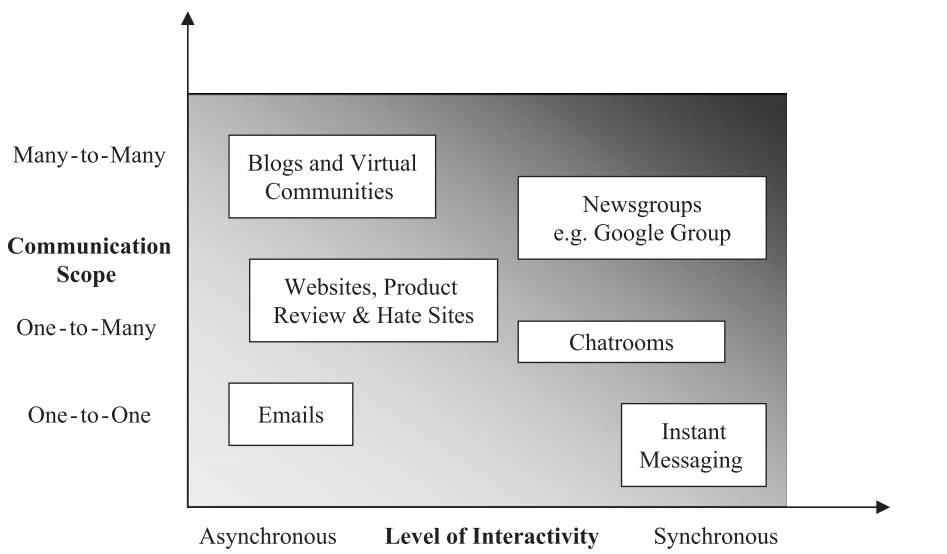
\includegraphics[width=\textwidth]{theoretische_grundlangen/Typologie_von_eWOM}
		\caption[Die Typologie von eWOM]{Die Typologie von {\ac{eWOM}} (Quelle:\citealp{Litvin2008})}
		\label{fig:typologieVoneWOM}
	\end{center}
\end{figure}

Diese Typologie meint deutlich, dass die \ac{OCRs} nur ein Unterbereich des \ac{eWOM}s sind. In der Dimension des Kommunikationsbereich sind \ac{OCRs} mengenwertig, und in Dimension der Interaktivität asynchron. Deshalb ist die Definition der \ac{OCRs} in dieser Arbeit nach \citet{Hennig-Thurau2004a}:

\textbf{``Online Consumer Review is any positive or negative statement made by potential, actual, or former customers about a product or company, which is made available to a multitude of people and institutions via the Internet''}

Diese Definition unterscheidet \acl{OCRs} deutlich von \ac{eWOM}. Für diese Definition ist es wichtig, die Gefühle von den Reviews, die von der Kunden gemacht werden, zu identifizieren. 

Nach \citet{Shrihari2012}, werden die \ac{OCRs} in zwei Gruppen unterteilt: qualitative und quantitative \ac{OCRs}. Qualitative \ac{OCRs} sind die schriftliche Beschreibungen der Kunden. Und die Quantitaive \ac{OCRs} sind die Werte der Online Ratings des Produkts. Im Falle eines quantitativen Online Consumer Review ist der Kunde gezwungen, seine oder ihre Auswertung in einer einzigen Bewertung oder Grad zusammenzufassen, und die einzelne Ratings von Kunden werden in der Regel zusammen in eine Auswertungsstatistik gebündelt. \citep{Kostyra2015}

Abbildung \ref{fig:beispiel_ocr} ist ein Beispiel des Online Consumer Review aus Amazon. Der quantitative Teil des Reviews im Beispiel ist diese ``drei Sterne''in dem ``Fünf-Sterne-Rating-System'' in Amazon. Und die anderen schriftlichen Teilen sind das qualitative Online Consumer Review.

\begin{figure}[htb]
	\begin{center}
		
\includegraphics[scale=1.0]{theoretische_grundlangen/ocr_amazon}
		\caption[Ein Beispiel von OCRs]{Ein Beispiel von \ac{OCRs}, (Quelle: \href{http://www.amazon.de/}{Amazon.de})}
		\label{fig:beispiel_ocr}
	\end{center}
\end{figure}

Gemäß \citet{pradeep2010the} kann ein Online Consumer Review in die folgenden drei Attribute zerlegt werden:
\begin{enumerate}
	\item \textbf{Volumen} ist die Gesamtzahl der Ratings von den Kunden.
	\item \textbf{Valenz} ist die durchschnittliche Rating von den Kunden, und repräsentiert die durchschnittliche Kundenzufriedenheit.
	\item \textbf{Varianz} ist die Variation der Ratings entlang der Rating-Skala und ist durch die Anzahl der Kundenbewertungen für jeden Valenzniveau beobachtbar. Varianz stellt den Grad der Meinungsverschiedenheiten oder Heterogenität der Auswertungen von den Kunden dar.
\end{enumerate}
%%=============================================================
\subsection{Forschungsstand zu Online Consumer Reviews}
%% seit wann werden diese verstärkt behandelt?
Es gibt zwei unterschiedliche Forschungswege \ac{OCRs} zu studieren. Viele Wirtschaftswissenschaftler glauben, dass die \ac{OCRs} eine Form von \ac{eWOM} ist, und damit studieren sie die \ac{OCRs} ähnlich wie \ac{eWOM}. \ac{eWOM} wird außerdem noch als ein Synonym von \ac{OCRs} benutzt \citep{SerraCantallops2014}.

%%Obwohl \ac{OCRs} ein Unterbereich unter \ac{eWOM} ist, haben die heutzutagen Untersuchungen sie nicht deutlich unterscheidet. 

Der Begriff \ac{eWOM} hat sich aus \ac{WOM} entwickelt, die auf Deutsch Mund-zu-Mund heißt, ist ein Faktor, das in dem Prozess des Treffens der Entscheidungen von Kunden wichtig ist \citep{SerraCantallops2014}. \citet{harrison2001measurement} definiert \ac{WOM} als ``\emph{informal, person-to-person communication between a perceived noncommercial communicator and a receiver regarding a brand, a product, an organization, or a service.}'' und \citet{dick1994customer} als ``\emph{a volitional post-purchase communication by consumers.}'' Die meisten Studien analysieren WOM als Faktor, der zu einem größeren oder geringeren Grad den Verbraucher in der Auswahl von Produkten und Dienstleistungen beeinflusst \citep{SerraCantallops2014}.

Da sich die Kommunikationsumgebung geändert hat, wurde die Forschung über \ac{WOM} aktualisiert \citep{Vilpponen2006}. Zwar ist \ac{eWOM} ähnlich wie die traditionelle Form des \ac{WOM}, doch mit den einigen einzigartigen Eigenschaften. Häufiger ist \ac{eWOM} zwischen Menschen zu beobachten, die wenig oder gar keine vorherige Beziehung zueinander haben (zum Beispiel Fremde) und kann anonym sein \citep{Dellarocas2003, goldsmith2006measuring, sen2007you}. Diese Anonymität ermöglicht es den Verbrauchern, bequemer ihre Meinungen mitzuteilen, ohne Offenlegung ihrer Identität \citep{goldsmith2006measuring}. Die Bereitschaft von Einzelpersonen, ihre Meinung auszudrücken, kann durch die bestehenden öffentlichen Meinungen auf der Webseite beeinflusst werden, und zur gleichen Zeit wollten Personen auch, die öffentliche Meinung durch ihre Meinungen zu beeinflussen \citep{Hong2011}. Dieses Phänomen ist viel häufiger in den Plattformen, die viele \ac{OCRs} haben, weil die \ac{OCRs} mengenwertig sind.

Diese einzigartigen Eigenschaften der \ac{OCRs} ermutigen die Verbraucher, ihre Meinungen mit mehreren anderen Verbrauchern zu teilen, so dass das Volumen der \ac{OCRs} sich erhöht \citep{chatterjee2001online}. Dadurch gibt es eine größere Wahrscheinlichkeit, dass die Verbraucher andere Verbraucher mit Fachwissen über das Produkt in den Plattformen finden könnten \citep{duhan1997influences}. 

Ein anderer Forschungsweg für die frühere Studien zum Verständnis der \ac{OCRs} ist durch Online Rückkopplungsmechanismen (\ac{i.e.} Online-Feedback-Mechanismus) \citep{Dellarocas2003}. Online Rückkopplungsmechanismen, die auch als Reputation-Systeme bekannt sind \citep{resnick2000reputation}, sind unter Verwendung von bidirektionalen Kommunikationsfunktionen des Internet, künstlich die groß angelegte \ac{WOM}-Netzwerke zu konstruieren, in denen die Menschen Erfahrungen und Meinungen über die vielfältigen Themen teilen können, inklusiv Unternehmen, Produkte, Dienstleistungen, und sogar Weltereignisse \citep{Dellarocas2003}.

Zum Beispiel, ist das Online-Feedback-System von eBay ein der am besten studierte Online Rückkopplungsmechanismen. Dieses System sammelt die Bewertungen von den Käufern und auch von den Verkäufern nach jedem Geschäft \citep{resnick2002trust}. Abbildung \ref{fig:feedback_ebay} zeigt ein Beispiel von einem Käufer und Verkäufer. \citeauthor{resnick2002trust} haben herausgefunden, dass diese Feedbacks fast immer positiv sind, und es gab eine hohe Korrelation der Feedbacks zwischen Käufern und Verkäufern.

\begin{figure}[htb]
    \minipage{\textwidth}
    
\includegraphics[width=\linewidth]{theoretische_grundlangen/feedback_ebay_kaufer}
    \endminipage\hfill
    \minipage{\textwidth}
    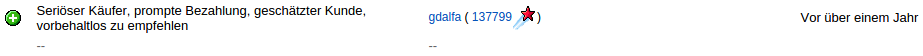
\includegraphics[width=\linewidth]{theoretische_grundlangen/feedback_ebay_verkaufer}
    \endminipage 
    \caption[Ein Beispiel von Online Rückkopplungsmechanismen]{Ein Beispiel von Online Rückkopplungsmechanismen (Quelle: \href{http://feedback.ebay.de/}{eBay.de})}
    \label{fig:feedback_ebay}
\end{figure}

Es gibt Anzeichen dafür, dass die Menschen zunehmend Meinungen in solchen Systemen schreiben wollen, um eine Vielzahl von Entscheidungen zu treffen, die sind, von welcher Film anzusehen, bis in welcher Aktien zu investieren \citep{guernsey2000suddenly}. Erst vor fünf Jahren haben die gleichen Leute in erster Linie diese Entscheidungen getroffen, die auf Werbungen oder professionellen Beratungen basiert sind \citep{Dellarocas2003}. 

Es ist interessant zu beobachten, dass die Forschungen durch diesen Weg die gleichen Ergebnisse wie \citet{duhan1997influences, Hong2011} hervorgebracht haben. Die beiden Forschungswege werden in Abbildung \ref{fig:forschungswege} gezeigt.
\begin{figure}[htb]
	\begin{center}
		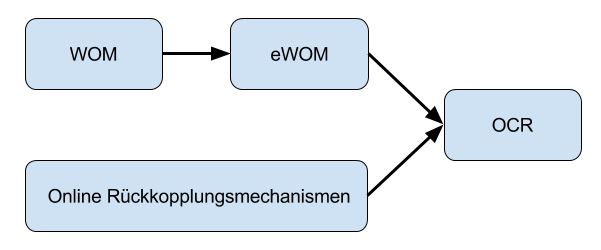
\includegraphics[width=\textwidth]{theoretische_grundlangen/forschungswege}
		\caption[Die beiden beobachteten Forschungswege über OCRs]{Die beide beobachtete Forschungswege über \ac{OCRs} (Quelle: Eigene Darstellung)}
		\label{fig:forschungswege}
	\end{center}
\end{figure}

Die bisherige Forschung über \ac{OCRs} fokussiert sich im Allgemeinen auf zwei Forschungsrichtungen. Einerseits sind die Faktoren, die sich auf die Erzeugung von Kommentaren beziehen; und auf der anderen Seite ist die Wirkung der Kommentare \citep{SerraCantallops2014}. In Abschnitt \ref{sec:erzeugungsfaktoren} und \ref{sec:auswirkung} werden die beiden Forschungsrichtungen diskutiert.
%%============================================================
\subsection{Motive für das Schreiben von Online Consumer Reviews} \label{sec:erzeugungsfaktoren}
%%===========================================================
In Bezug auf die Motive von \ac{OCRs}, zeigen die meisten der untersuchten Studien Aspekte wie ``Service-Qualität und Zufriedenheit'', ``Fehler und Wiederherstellung'', ``Unzufriedenheit der Kunden'' und ``Sinn für die Zugehörigkeit der Gemeinschaft'' als Hauptmotive der Verbraucher für das Schreiben der Bewertungen \citep{Swanson2009critical, Kim200951, Sun2011isthere, SanchezGarcia20111397, Nusair2011833}. Diese Studien identifizieren eine direkte Beziehung zwischen Zufriedenheit oder Unzufriedenheit mit positiven oder negativen Bewertungen und ist ein ziemlich offensichtliches und vorhersehbares Konsumverhalten \citep{SerraCantallops2014}. Einige Autoren setzen die Themen bezüglich ``Engagement'', ``soziale Identität'', ``Erwartungen vor dem Kaufen'', und ``Kunden begeistert'' als wichtige Aspekte bei den Motiven \citep{crotts2009measuring, Casalo2010898, bronner2010vacationers}.

\citet{Hennig-Thurau2004a} machte eine Zusammenfassung von allen Motiven durch die Definition von \ac{WOM}. Durch die Theorien von \citet{dichter1966word, engel1993consumer, sundaram1998word} werden die Motive der Erstellung von \ac{OCRs} in 11 Faktoren von \citeauthor{Hennig-Thurau2004a} unterteilt. Die sind: Sorge um andere Verbraucher; Unterstützung von Unternehmen; Erhalten von den sozialen Vorteilen; Ausübung von Macht; Postkaufberatung suchen; Selbstverbesserung; wirtschaftlichen Erfolg; Komfort bei der Suche nach Wiedergutmachung; Unterstützung der Plattformbetreiber; positive Emotionen auszudrücken; und negativen Gefühle zu erleichtern.

Diese 11 zusammenfassenden Faktoren wurden von rund 2000 Verbraucher, die aktiv auf den deutschen Web-basierten Meinungsplattformen sind, empirisch geprüft. Die Motivation, Sorge um andere Verbraucher, ist das Hauptmotiv. Danach folgen die wirtschaftliche Anreize und positive oder negative Gefühle auszudrücken. \citep{Hennig-Thurau2004a}
%%noch ein bisschen kann man schreiben, wenn benötigen.
%%===========================================================
\subsection{Wirkungen von Online Consumer Reviews} \label{sec:auswirkung}
%%===========================================================
Es gibt viele Aspekte über die Wirkungen von \ac{OCRs} in Marketing. \citet{Dellarocas2003} findet sich eine Auflistung von Forschungen, die Wirkungen der Valenz von \ac{OCRs} aufzeigen, (das heißt, dass die \ac{OCRs} positiv, negativ oder neutral sind),  mit der Maßnahme Online Rückkopplungsmechanismen. Die Tabelle \ref{tab:onlinefeedback} zeigt diese Forschungen.
%\begin{table}[h] 
%\centering
\begin{longtable}{p{.15\textwidth} p{.20\textwidth}  p{.55\textwidth}}
\hline
Quelle& Untersuchungs-objekte& Ergebnisse\\ \hline
\citet{ba2002evidence}& Musik, Software& Positive Bewertungen erhöhen den geschätzten Preis, aber negativen haben keinen Effekt.\\ \hline
\citet{bajari2003winner}& Münzen& Sowohl positive als auch negative Bewertungen beeinflussen die Wahrscheinlichkeit des Eintritts der Käufer in die Auktion, aber nur positive Bewertungen hatte einen signifikanten Einfluss auf den Endpreis. \\ \hline
\citet{eaton2002valuing}& Elektrische Gitarren& Negative Bewertung reduziert die Wahrscheinlichkeit auf den Verkauf, aber nicht auf den Preis der verkauften Produkte.\\ \hline
\citet{houser2006reputation}& Pentium-Chips& Positive Bewertung erhöht den Preis; negativer Kommentar reduziert Preis.\\ \hline
\citet{kalyanam2001returns}& Palm Pilot PDAs& Positive Bewertung erhöht den Preis; negativer Kommentar reduziert Preis.\\ \hline
\citet{kauffman2000running}& Münzen& Keine besonderen Wirkungen, aber negativer Kommentar erhöht den Preis in der univariaten Analyse vielleicht.\\ \hline
\citet{lee2000effect}& Computer-Monitore und Drucker& Negativer Kommentar reduziert den Preis, aber nur für die gebrauchte Ware.\\ \hline
\citet{livingston2005valuable}& Golfklubs& Positive Bewertung erhöht sowohl die Wahrscheinlichkeit für den Verkauf als auch für den Preis; Effekt ausläuft, sobald ein Datensatz etabliert.\\ \hline
\citet{lucking2007pennies}& Münzen& Keine Auswirkung von positiver Bewertung; negativer reduziert den Preis.\\ \hline
\citet{melnik2002does}& Goldmünzen& Positive Bewertung erhöht den Preis; negativer Kommentar reduziert den Preis.\\ \hline
\citet{mcdonald2002reputation}& Puppen& Mehrere Bewertungen (positive oder negative) erhöht den Preis. \\ \hline
\citet{resnick2002trust}& MP3-Player, Beanie Babies& Beide Formen des Kommentars beeinflussen die Wahrscheinlichkeit für den Verkauf, aber es gibt keine Abhängigkeit auf den Preis.\\ \hline
\citet{resnick2006value}& Weinlesepostkarten& Geringe Wirkung von den kleinen Menge des negativen Kommentars.\\ \hline
\caption[Auswirkung der Valenz von OCRs]{Auswirkung der Valenz von \ac{OCRs}, (Quelle: \citealp{Dellarocas2003})}\\
\label{tab:onlinefeedback}
%\tabularnewline
\end{longtable}
%\end{table}

Die Auswirkungen der \ac{OCRs} wurden in den letzten Jahren sowohl aus der Unternehmenssicht als auch der Konsumentensicht analysiert. \citet{SerraCantallops2014} hat eine Zusammenfassung dafür im Bereich Hotelleitung gemacht, und fand, dass die Hauptauswirkungen von \ac{OCRs} aus der Konsumentensicht: Entscheidungsprozess, Glaubwürdigkeit, Risikoreduktion, Produktakzeptanz, Loyalität, Markenbewusstsein, \ac{usw} sind. Aus der Unternehmenssicht sind die Auswirkungen häufig: Qualitätskontrolle und neue Produkte, Ertragsmanagement, Kundeninteraktion und Wiederherstellung, Kommunikation, die sie sich auf das Ziel konzentrieren, spezifische Marketing-Strategien, Online-Reputation, und Loyalitätserzeugung. Die Abbildung \ref{fig:auswirkungvonOCR} stellt die Ergebnisse graphisch dar.
\begin{figure}[htb]
\centering
	\minipage{0.5\textwidth}
	\includegraphics[width=\linewidth]{theoretische_grundlangen/impactKS}
	\endminipage\hfill
	\minipage{0.5\textwidth}
	\includegraphics[width=\linewidth]{theoretische_grundlangen/impactUS}
	\endminipage\hfill
\caption[Auswirkungen der OCRs aus Konsumenten- und Unternehmenssicht]{Auswirkungen der \ac{OCRs} aus Konsumenten(Links)-und Unternehmenssicht(Rechts) (Quelle: \citealp{SerraCantallops2014})}
\label{fig:auswirkungvonOCR}
\end{figure}

\citet{Cheung2012} beobachtete, dass es noch keine Forschung aus der Unternehmenssicht bis zum Jahr 2004 gab. Aber aus der Konsumentensicht gibt es schon ab 2001 Studien über \ac{OCRs} . Im Jahr 2008 gab es insgesamt 15 Studien,  66\% davon waren aus der Konsumentensicht, aber im Jahr 2010 war die Zahl nur 2, jedoch gab es 10 Studien aus der Unternehmenssicht.\citep{Cheung2012} Die Abbildung \ref{fig:timeline} zeigt die von \citeauthor{Cheung2012} festgestellte Zeitachse von \ac{OCRs}.

\begin{figure}[htb]
	\begin{center}
		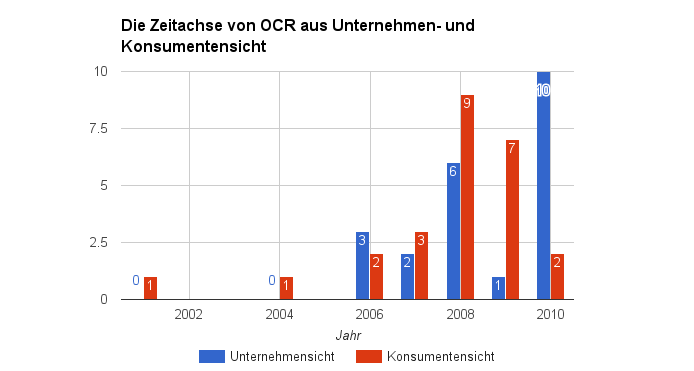
\includegraphics[width=\textwidth]{theoretische_grundlangen/timeline}
		\caption[Die bemerkte Zeitachse von OCRs]{Die bemerkte Zeitachse von \ac{OCRs} (Quelle: \citealp{Cheung2012})}
		\label{fig:timeline}
	\end{center}
\end{figure}

Einige Studien, die die Auswirkungen der \ac{OCRs} studieren, fokussieren sich auf die qualitativen und quantitativen Aspekten. In den qualitativen Bewertungen ist es dem Kunden völlig frei, wie Sie beschreiben, kritisieren und das Produkt bewerten \citep{Jimenez2013226}. Im Falle einer quantitativen Bewertung ist der Kunde gezwungen, seine oder ihre Auswertung in einer einzigen Bewertung oder Grade zusammenzufassen, und die Einzelbewertungen von Kunden werden in der Regel in eine Auswertungsstatistik zusammengefasst \citep{Kostyra2015}.

Diese Studien aber analysieren nur aus quantitativer Sicht. Sie haben schon viel über die Valenz (beispielsweise: 5 Sterne-Rating in Amazon), Volumen (Anzahl der \ac{OCRs}), und Varianz (zeigt den Grad der Meinungsverschiedenheiten der Kunden) der \ac{OCRs} in der quantitativen Aspekte studiert. Was der Kunde schreibt, ist für die Studien unwichtig. Tabelle \ref{tab:quantitativOCR} zeigt die Ergebnisse dieser Studien.


\begin{longtable}{p{.15\textwidth} p{.20\textwidth}  p{.55\textwidth}} 
\hline
Quelle& Untersuchungs-objekte& Ergebnisse\\ \hline
\citet{yubo2011online}& Kameras& Negative Bewertungen haben stärkere Auswirkung als positiven. \ac{OCRs} zeigen eine abnehmende Auswirkung über die gesamte Lebensdauer.\\ \hline
\citet{judith2006the}& Bücher& Bessere Valenz von \ac{OCRs} werden den Umsatz für Amazon verbessern, aber nicht für Barnes \& Noble. Volumen verbessert den Umsatz für Amazon.\\ \hline
\citet{pradeep2010the}& Filme& Valenz ist wichtig für die Vorhersage des Umsatzes, aber nicht Volumen oder Varianz.\\ \hline
\citet{eric2006when}& Bier& Varianz ist signifikant mit dem Umsatzwachstum korreliert. Durchschnittliche Valenz ist signifikant.\\ \hline
\citet{cui2012effect}& Videospiele und Elektronikläden& Valenz und Volumen sind signifikant. Valenz hat eine stärkere Auswirkung als Volumen, um Waren zu suchen. Aber wenn Kunde Erfahrung über die Ware hat, wechselt diese Beziehung.\\ \hline
\citet{Dellarocas200723}& Filme& Valenz und Volumen zeigen eine signifikante Beziehung mit dem zukünftigen Schalterverkauf.\\ \hline
\citet{Dhar2009300}& Musik& Valenz ist signifikant für eine Woche-voraus-Vorhersage in einem Modell mit festen Effekten. Volumen wird nicht implementiert.\\ \hline
\citet{Duan20081007}& Filme& Valenz hat keine Effekte für den Umsatz, aber Volumen ist signifikant.\\ \hline
\citet{nga2013the}& DVD& \ac{OCRs} haben eine signifikante Auswirkung auf die schwach aufgeladene Marken, aber keine signifikante Auswirkung auf die starken.\\ \hline
\citet{wendy2011the}& Bath, Duft, und Schönheitspflege& Es gibt positive direkte Effekte der Valenz auf den Umsatz. Keine direkte Effekte von Varianz und Volumen auf den Umsatz.\\ \hline
\citet{monic2012how}& Bücher& Auswirkung der Volumen ist positiv und signifikant für Amazon. Valenz ist bezeichnend für Amazon, aber nicht für  Barnes \& Noble. Interaktion mit der Valenz und Varianz ist signifikant.\\ \hline
\citet{Zhu2010}& Konsolenspiele& Valenz und Varianz sind signifikant für weniger bekannte Spiele mit einem Online-Modus. Volumen ist bezeichnend für Spiele mit dem Online-Modus.\\ \hline
\citet{Kostyra2015}& eBook-Reader& Valenz hat eine positive direkte Wirkung auf die Produktwahl. Volumen moderiert nur hohen Valenz. Varianz moderiert hohe und mittlere Valenz negativ.\\ \hline
\caption[Ein Überblick über die Literature in quantitativer Aspekte]{Ein Überblick über die Literature in quantitativer Aspekte, in Anlehnung an \citet{Kostyra2015}}
\label{tab:quantitativOCR}
\end{longtable}

Es ist schwer eindeutige Zusammenhänge zu kommen, obwohl Wirtschaftler schon so viele Studien und Forschungen gemacht haben. Es wird einfach beobachtet, dass viele Ergebnisse in Tabelle \ref{tab:onlinefeedback} und \ref{tab:quantitativOCR} im Konflikt stehen, auch über das gleiche Untersuchungsobjekt oder in dem gleichen Bereich. Beispielsweise findet \citet{pradeep2010the}, dass Valenz wichtig für die Vorhersage des Umsatzes ist, aber Volumen oder Varianz nicht. Dagegen sagt \citet{Duan20081007}, dass Valenz keine Effekte für den Umsatz hat, aber Volumen ist signifikant.\citet{kauffman2000running} findet dass negative Kommentare den Preis erhöhen, aber \citet{lucking2007pennies} ist da ganz anderer Meinung. 

Gründe für diese im Konflikt stehende Ergebnisse sind vielfältig. Es gibt meist die folgende drei verschiedene Gründe:
\begin{itemize}
	\item Die Qualität und Glaubwürdigkeit zu bestimmen ist schwer für die potenziale Kunden, weil die \ac{OCRs} anonym sind \citep{chatterjee2001online, schindler2005published}.
	\item Wegen der Anonymität haben einige Verkäufer versucht, \ac{OCRs} zu verbessern durch die wirtschaftliche Anreize an die guten Bewertungen, und auch durch das Veröffentlichen ihrer eigenen Kommentaren \citep{chatterjee2001online}
	\item Viele Konsumenten geben eine quantitative Bewertung, die trotz seiner oder ihrer Meinung (qualitative Bewertung) nicht passend ist. Das heißt, dass die quantitative Bewertungen nicht so glaubwürdig, wie viele Wirtschaftler geglaubt haben, sind.
\end{itemize}

Aus dieser Gründen lesen die Konsumenten häufig eine Vielzahl von \ac{OCRs} durch, um die Qualität und Glaubwürdigkeit der Online-Information zu bestimmen \citep{greer2003evaluating}. Eine Umfrage ergab, dass 90\% der Verbraucher die \ac{OCRs} lesen, während 83\% von ihnen stimmt zu, dass \ac{OCRs} ihre Kaufentscheidungen beeinflussen würden \citep{lu2015understanding}. Laut \citet{Zhu2010} hatten die \ac{OCRs} einen stärkeren Einfluss auf weniger beliebte Produkten.

Und auf diese Gründe entsteht ein Bedarf für Unternehmen, Plattformbetreiber, Wirtschaftswissenschaftler, und auch die Konsumenten, die qualitative Kommentaren zu verstehen und zu analysieren. Das heißt, dass es eine theoretische Studie ist erforderlich, um das Wissen von Meinungen der Menschen gegenüber dieser Produkte, Services oder Attribute, zu extrahieren \citep{Khan2011}. 
%%===========================================================
\subsection{Online Consumer Reviews im Textileinzelhandel} \label{sec:OCRsinTextil}
%%===========================================================
Ein Erfahrungsgut ist es, das nur erst nach dem Kauf des Produkts ausgewertet werden kann \citep{nelson1970information}. Einige Erfahrungsgüter wie Kleidung sind nun weitgehend, die über das Internet verkauft \citep{Lee2009a}. Der Einkauf der Kleidung erfordert ``Touch-and-Feel'' Auswertungen in einer Vor-Kaufphase. Da die Menschen die sensorischen Informationen unterschiedlich empfangen und verarbeiten, können sie unterschiedlichen Wahrnehmungen des gleiche Produkts haben \citep[p.~151]{armstrong2014principles}. Frühere Studien haben mehrere Faktoren und Hinweise, die die Sicht der Verbraucher auf der Qualität der Kleidung beeinflussen, identifiziert.

Viele Studien kategorisieren die Attribute, die die Wahrnehmungen der Verbraucher bestimmen oder beeinflussen, in zwei allgemeine Typen - äußere und innere. Innere Attribute beziehen sich auf eigenen Eigenschaften des Produkts, die ohne das tatsächliches Produkt nicht geändert werden können, während die äußeren Attribute kein Teil des Produktes sind, sondern relevant \citep[p.~167]{olson1972proceedings}.

\citet{eckman1990toward} haben vor 1990 die Erkenntnisse zusammengefasst, dass der Preis und die Marke die am häufigsten genannte äußere Kriterien waren, während Produktzusammensetzung (Stil, Farbe/Design, Stoff, Aussehen) und Leistung (Pflege, Passform, Haltbarkeit und Komfort) die am häufigsten genannte innere Kriterien waren. Farbe/Muster, Stil, Stoff, Passform und Aussehen wurden als der wichtigsten Faktoren in dem In-Store-Kaufprozess der Kleidung identifiziert \citep{eckman1990toward}. \citet{forsythe1991effect} stellte fest, dass die Verbraucher die Auswertungen und Eindrücke von Kleidung gebildet waren, durch die Verwendung von äußeren Faktoren (Marke, Preis, \ac{usw}.) und inneren Kriterien, Design, Stil, die Konstruktionsdetails, die hauptsächlichen Kriterien waren \citep{eckman1990toward}. \citet{fiore1992intrinsic} konzentrierten ihre Studie über die innere Signale und haben gefunden, dass die ästhetische Attribute wie das Layout (Design) und Stoff am wichtigsten waren. Mit offenen Fragen und Content-Analyse, entdeckten \citet{lennon1994categorization}, dass ästhetische Attribute die meisten identifiziert wurden, nach Leistung, äußeren Attributen und Nützlichkeit.

\citet{abraham1995consumers} verwendeten Fokusgruppen-Interviews, um eine vollständige List der Attribute einschließlich physischer Erscheinung (Stoff, Farbe/ Muster/ Textur, Bau und Styling), die körperliche Leistungsfähigkeit (Stoff, Farbe, Pflege, Verarbeitung und Kleidungsstück), expressive Attribute (``Schaut auf mich'', Angemessenheit, Kommentare von anderen) und äußere Attribute (Marke, Preis, Geschäft, Herkunftsland, und Service) zu erzeugen. Die physische Erscheinung wurde in meistens genannt \citep{abraham1995consumers}. Basierend auf dieser Liste, haben \citet{abraham1995perceptions} eine weitere Studie über die Sicht der Verbraucher in den Vor- und Nach-Kaufphase gemacht, und festgestellt, dass Stoff und Bekleidungskonstruktion, Stil, Pflege, Verarbeitung und Kosten zu den wichtigsten Attributen im Allgemeinen gehörten.

\citet{forsythe1996dimensions} untersucht dieses Thema durch Einkaufszentrum mit realen Produkten und realen Einkaufssituationen, und stellten fest, dass die Robustheit/ Haltbarkeit (inklusiv Stoffkonstruktion im Lieferumfang) und Stil/ Ästhetik (Design, Styling, Aussehen) die Schlüssedimensionen waren, die das Bewusstsein der Verbraucher am meisten beeinflussen. Haltbarkeit und Pflege waren wichtige Entscheidungsfaktoren, aber tragen nicht zu der Qualitätsbewertung bei. Dieses Ergebnis war im Widerspruch zu den meisten früheren Studien.

\citet{swinker2006understanding} haben herausgefunden, dass die Ästhetik der wichtigste Faktor war, gefolgt von Leistung (Haltbarkeit, Versorgung, \ac{usw}.) und äußeren Kriterien. Aber keine innere Kriterien wurden identifiziert, aufgrund es Fehlen von momentan vorliegender Kleidung. \citet{abraham1995consumers} und \citet{swinker2006understanding} stimmten zu, dass die Verbraucher immer multidimensionalen Kriterien verwenden, um die Kleidung zu bewerten.

Viele andere Studien berücksichtigten dieses Thema in verschiedenen Stufen. \citet{rosenau2014apparel} definierten die Qualitätsmessung der Verbraucher als ``zweistufiges Verfahren'' (p.263-264). Sie meinten dass Ästhetik (Stil, Farbe, Stoff, Zierteile und passen) und Konstruktionsdetails wie Nähte, Stiche und Mustererkennung zuerst bewertet wurden während die Haltbarkeit, Komfort, Pflege und das Aussehen in der zweiten Beurteilung waren. Viele Forscher haben festgestellt, dass die Verbraucher das Produkt mit dem Preis (Kosten) bewerten wurden \citep{keller2011strategic, kadolph2007quality}, aber die Ergebnisse für die Wichtigkeit der Kosten waren inkonsistent \citep{lu2015understanding}. Laut \citet{Goldsmith2002}, standen die demographischen Variablen wie Alter und Geschlecht in keinem Zusammenhang mit dem Online-Bekleidungseinkauf.

Basierend auf früheren Studien, werden drei allgemeine Attributkategorien - Ästhetik, Performance, und äußere Attribute in dieser Studie verwendet:
\begin{enumerate}
	\item \textbf{Ästhetik} inklusiv Farbe, Muster, Stil (Sihouette, Modebewusstsein), Verarbeitung (Stiche, Nähte und Konstruktinsdetails), Vielseitigkeit (Anpassungsfähigkeit) und das Aussehen (wie das Kleidungsstück sieht für den Verbraucher).
	\item \textbf{Performance} inklusiv Passform (Große), Komfort, Haltbarkeit und Pflege.
	\item \textbf{Äußere Attribute} sind Marke, Preis und Service.
\end{enumerate}

Diese drei Kategorien sind die Attribute, worüber die Kunden \ac{OCRs} über die Kleidung schreiben wollen. Als \citet{hu2008online} erwähnt, werden die \ac{OCRs} von Verbrauchern eine Hauptquelle für die Verbraucher als auch Unternehmen, um die Informationen über das Produkt zu zugreifen. Differenzen in den Kulturen haben ein unterschiedliches Konsumverhalten in verschiedenen Ländern zu Folge \citep{keller2011strategic}. Dieses Verhalten spiegelt sich auch im Schreiben der \ac{OCRs} wider. Die kulturellen Differenzen werden im Abschnitt \ref{sec:relevante_forschungen} diskutiert.
%%===========================================================
\section{Sentiment Analyse}
%%===========================================================
\subsection{Definition} \label{SAdefinition}
%%==========================================================
Sentiment Analyse (auch als Opinion Mining bekannt \citep{tapia2014twitter,duenassentiment}) ist ein Teilgebiet des Text Minings, mit der Hauptaufgabe, die Meinungen von Web-Benutzer generierten Inhalten zu extrahieren \citep{Balazs2016}. Es existieren viele Definitionen, die verschiedene Bereiche und Ebenen der Granularität präsentieren \ac{i.e.}:
\begin{description}
	\item[\citet{Wilson:2005:RCP:1220575.1220619}] ``the task of identifying positive and negative opinions, emotions and evaluations''.
	\item[\citet{Feldman:2013:TAS:2436256.2436274}] ``the task of finding the opinions of authors about specific entities''.
	\item[\citet{vinodhini2012sentiment}] ``tracking the mood of the public about a particular product or topic''.
	\item[\citet{6468032}] ``the task of polarity classification''.
\end{description}
In dieser Arbeit, wird die Meinung (\ac{i.e.}:``Opinion'') laut der Definition von \citet{liu2010sentiment}, als ein Tupel definiert:

$$(e_i, a_{ij}, s_{ijkl}, h_k, t_l)$$

, in dem die Bedeutungen sind:
\begin{description}
	\item[$e_i$] ist die Entität der $i$ten Meinung.
	\item[$a_{ij}$] ist das $j$te Attribut von $e_i$.
	\item[$h_k$] ist der $k$ten Autor der Meinung.
	\item[$t_l$] ist das Zeitpunkt wann die Meinung abgegeben wird.
	\item[$s_{ijkl}$] ist die Polarität der Meinung gegenüber das Attribut $a_{ij}$ von der Entität $e_i$ bei dem Autor $h_k$ am Zeitpunkt $t_l$.
\end{description}
%%Deshalb ist die Hauptaufgabe von Sentiment Analyse: (\ac{i.e.})
%%\begin{description}
%%	\item[$s_{ijkl}$] ist die Polarität der Meinung gegenüber das Attribut $a_{ij}$ von der Entität $e_i$ bei dem Autor der Meinung $h_k$ am Zeitpunkt $t_l$.
%%\end{description}
Deshalb ist die Hauptaufgabe von Sentiment Analyse: (\ac{i.e.})

\textbf{``to find all the opinion tuples $(e_i, a_{ij}, s_{ijkl}, h_k, t_l)$ within a document, collection of documents (called corpus) or across many corpora.''} \citep{liu2010sentiment}

Diese Polarität $s_{ijkl}$ kann sowohl als positiv, negativ oder neutral, als auch numerisch dargestellt werden \citep{Balazs2016}. Wie zum Beispiel in dieser Arbeit wird 1 eine sehr negative Meinung sein, während 5 eine sehr positive Meinung ist. Auch wenn die Analyse nicht so viele Detailstufen erfordert, könnten die Attribute einer Entity entfallen und durch $GENERAL$ statt $a_{ij}$ bezeichnet werden \citep{Balazs2016}.

Es gibt noch andere Definitionen, wie die in \citet{neviarouskaya2010} präsentiert wird, in dem die Autoren versuchen, emotionale Zustände, wie (\ac{i.e.}) ``anger'', ``fear'', ``joy'', oder ``interest'' nur in positiv oder negativ zu klassifizieren. In diesem Fall könnte das Modell von \citet{liu2010sentiment}, durch Hinzufügen eines anderen Elements in das Tupel, die Informationen darstellen. \citep{Balazs2016}
%%============================================
\subsection{Der Ablauf der Sentiment Analyse}
%%============================================
Der übliche Ablauf oder Prozess der Sentiment Analyse besteht aus einer Reihe von festgelegten Schritten \citep{Khan2014245,arora6734936,deyhaque2009}, die Datensammlung (\ac{i.e.} data acquisition), Texte-Vorverarbeitung (\ac{i.e.} text preprocessing), Kernprozess (\ac{i.e.} core process), Aggregation und Zusammenfassung der Ergebnisse und Visualisierung (\ac{i.e.} aggregation and summarization of results and visualization) sind. Abbildung \ref{fig:sentimentanalysesprozess} zeigt den ganzen Ablauf.
\begin{figure}[htb]
	\begin{center}
		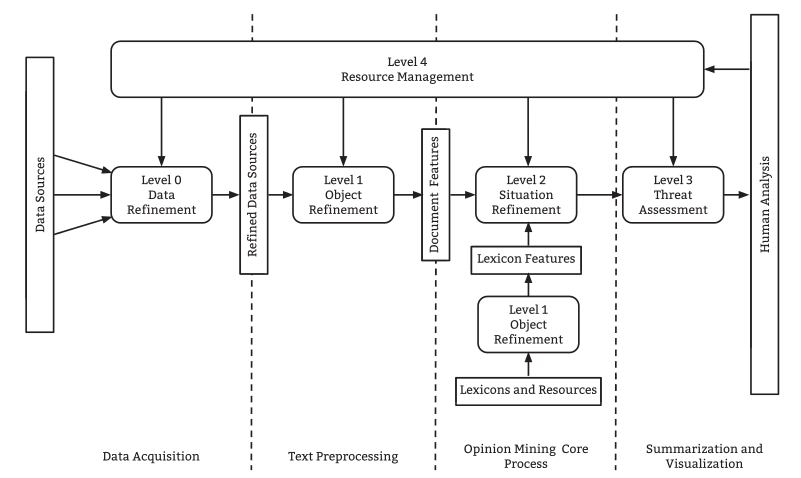
\includegraphics[width=\textwidth]{theoretische_grundlangen/sentimentanalysesprozess}
		\caption[Der Ablauf der Sentiment Analyse]{Der Ablauf der Sentiment Analyse (Quelle:\citealp{Balazs2016})}
		\label{fig:sentimentanalysesprozess}
	\end{center}
\end{figure}

In dieser Arbeit, werden die erste beide Schritten (\ac{bzw.} Datensammlung und Texte-Vorverarbeitung) in Kapitel \ref{datensammlung} diskutiert. Insbesondere wird der Kernprozess von Sentiment Analyse in Abschnitt \ref{SAkernprozess} dargestellt. Die anderen Schritten, sowie Zusammenfassung und Visualisierung der Ergebnisse, werden in Kapitel \ref{Kapital4empirischeErgebnisse} vorgestellt.
%%================================================
\subsection{Kernprozess} \label{SAkernprozess}
%%================================================
%%hier könnte mehr schreiben, wenn benötigen.
Mit zustimmender Popularität der Sentiment Analyse, gibt es viele unterschiedliche Ebenen der Analyse, \ac{bzw.} Dokument-Level, Satz-Level, Entität und Aspekt-Level \ac{usw} \citep{Balazs2016}. In dieser Arbeit, wird die Analyse von dem Dokument-Level durchgeführt.
\begin{description}
	\item[Dokument-Level:] Sentiment Analyse auf dieser Ebene versucht, Dokumente in positiv oder negativ zu klassifizieren. Formal kann die Aufgabe von Sentiment Analyse in Dokument-Level als modifizierte Version, die in Abschnitt \ref{SAdefinition} vorgestellt, definiert werden und entspricht der Suche nach dem Tupeln:
$$(-,GENERAL,s_{GENERAL},-,-)$$
, in dem die Entität $e$, der Autor, die Meinung $h$ und die Zeit $t$, wann die Meinung geschrieben wird, bekannt oder ignoriert sein wird, und das Attribut $a_j$ der Entität $e$ als $GENERAL$ entspricht. Das heißt, dass die Analyse nur die verallgemeinerte Polarität des Dokuments berücksichtigt. \citep{Balazs2016}

In dieser Arbeit wird jede Review vom Kunden als ein Dokument analysiert. Gleichzeitig werden auch jede vom Kunden vergebene Sterne notiert. Das bedeutet, dass jede Review Sterne und Polarität von Sentiment haben. Es wird verglichen, welche Unterschiede es in den beiden und zwischen Deutschland und China gibt.
	\item[Satz-Level:] Dieses Level ist analog zu dem vorherigen, da ein Satz als ein kurzes Dokument betrachtet werden kann. Allerdings wird ein zusätzlicher Vorverarbeitungsschritt erfordert, der aus Brechen des Dokumentes auf mehreren Sätzen besteht. Dieser Schritt stellt die ähnlichen Herausforderungen wie Tokenisierung, weil es Sprachen gibt, die nicht durch Punkte getrennt werden. \citep{Balazs2016}

In dieser Arbeit ist das Level nicht von Bedienung, weil die chinesischen Reviews meistens nur ein Satz eingewiesen werden, außerdem werden sie auch als ein Dokument schon in dem Dokument-Level analysiert. 
	\item[Entität und Aspekt-Level:] Dieses Level stellt die detaillierteste Ebene dar, auf der die Sentiment Analyse durchgeführt wird. Hier ist die Aufgabe nicht nur um die Polarität der Meinung, sondern auch sein Ziel (Entität, Aspekt odr beides) zu finden, damit die in Abschnitt \ref{SAdefinition} beschriebene 5-Tupel-Definition vollständig gilt. Sowohl auf Dokument-Level als auch Satz-Level funktioniert die Analyse gut, wenn die geprüften Texte nur eine Entität und Aspekt enthalten, aber sie sind ins Wanken geraten, wenn mehr vorhanden sind \citep{Feldman:2013:TAS:2436256.2436274}. Die Aspekt-basierte Sentiment Analyse versucht, dieses Problem zu lösen, durch Erfassen jedes erwähnten Aspekt im Text und in Verknüpfung mit einer Meinung. \citep{Balazs2016}

Die wichtigen Aspekte sind nach zwei Beobachtungen identifiziert: \citep{Yu2011}
\begin{enumerate}
	\item Die wichtigen Aspekte eines Produktes werden üblicherweise durch eine große Zahl von Verbrauchern kommentiert.
	\item Die Meinungen zu wichtigen Aspekten von Verbrauchern beeinflussen stark ihre allgemeine Meinung über das Produkt.
\end{enumerate}
Wegen der Besonderheiten des elektronischen Einzelhandels werden die Autoren der Reviews sinnlos sein, weil die andere Kunden die Autoren der Reviews nicht kennen könnten.
\end{description}
Es gibt zwei gut etablierte Ansätze, zur Durchführung des Kernprozesses der Sentiment Analyse. Einen davon ist der unbeaufsichtigte Lexikon-basierten Approach (\ac{i.e.} unsupervised lexicon-based approach), in dem sich der Prozess auf die, aus Sprachkenntnisse erhaltene, Regeln und Heuristiken stützt \citep{NLE:9479653}. Und der Andere ist der beaufsichtigte Maschine-Learning-Approach (\ac{i.e.} machine learning approach), in dem die Algorithmen die zugrundeliegenden Informationen lernen, die aus vorher kommentierten Daten sind, damit sie die neuen, unmarkierten Daten klassifizieren können \citep{Pang:2002:TUS:1118693.1118704}.
\begin{description}
	\item[Der unbeaufsichtigte Lexikon-basierte Ansatz:] (\ac{i.e.} ``the unsupervised lexicon-based approach'') auch als Semantik basierter Approach bezeichnet, versuchen, die Polarität des Textes unter Verwendung einer Reihe von den aus Sprachkenntnisse erhaltenen Regeln und Heuristiken zu bestimmen \citep{Balazs2016}. 

Die üblichen Schritte, um sie durchzuführen, sind: (1) jedes Wort und jeden Satz mit der entsprechenden Polarität mit Hilfe eines Lexikons zu klassifizieren. (2) die Analyse der Sentiment-Schiebern sowie deren Umfang (Verstärker und Verneinung) zu übernehmen.(3) Die adversative Klauseln (aber-Klauseln) durch das Verständnis, wie sie die Polarität beeinflusst zu behandeln, und dies in der letzten Sentiment-Score zu reflektieren \citep{Liu2012}.
%%historie nicht geschrieben.
	\item[Der beaufsichtigte Maschine Lerning Ansatz:] (\ac{i.e.} ``the supervised machine learning approach'') auch als statistische Methoden zur Sentiment-Klassifikation bekannt. Die bestehen aus Algorithmen, die zugrundeliegenden Muster von Beispieldatei lernen \citep{webpattern2010}, das heißt, die Daten, deren Klasse oder Label für jedes Exemplar bekannt sind, die später versuchen, neue, nicht-markierte Daten zu klassifizieren \citep{mitchell1997machine}.

Die üblichen Schritte bestehen aus Projektierung der Merkmale, um das Objekt, dessen Klasse prognostiziert wird, darzustellen, und dann mit ihrer Darstellung als Eingabe des Algorithmus \citep{Balazs2016}. Einige Merkmale, die in der Sentiment Analyse häufig verwendet werden, sind: Wortfrequenz, Wortart, die Stimmung der Wörter und Sätze, Regeln der Meinung, Sentiment-Schiebern und syntaktischen Abhängigkeit \citep{Liu2012, Joshi:2009:GDF:1667583.1667680}.
\end{description}
In dieser Arbeit wird die unbeaufsichtigte Methode verwendet. Einer der Vorteile der Verwendung davon ist, nicht mehr auf große Datenmengen für die Ausbildung der Algorithmen zu beruhen. Dennoch ist es notwendig, ein Sentiment-Lexikon zu erhalten oder zu erstellen. Die unbeaufsichtigten Methoden sind auch weniger domainabhängig als die beaufsichtigten Verfahren. In der Tat haben die in einer Domain ausgebildeten Klassifikationen konsistent schlechtere Performance in anderen Bereichen. \citep{aue2005customizing,blitzer2007biographies} 
%%======================================================
\subsection{Der konkrete Algorithmus im Dokument-Level}  \label{algorithmus}
%%======================================================
Wie es oben gezeigt wird, ist es wichtig, ein guten Sentiment-Lexikon zu erhalten. Die Genauigkeit der Polarität ist sehr abhängig von dem Sentiment-Lexikon für die unbeaufsichtigten Methoden. In dieser Arbeit wird das Lexikon von \citet{Remus2010} verwendet. Tabelle \ref{tab:LexikonInhalt} zeigt einen Überblick über den Inhalt des Lexikons.
% Please add the following required packages to your document preamble:
% \usepackage{multirow}
\begin{table}[htb]
\centering
\begin{tabular}{|l|l|l|l|}
\hline
                                                 &                & Positiv         & Negativ         \\ \hline
\multicolumn{1}{|c|}{\multirow{2}{*}{Adjektive}} & Stammform      & 784             & 698             \\ \cline{2-4} 
\multicolumn{1}{|c|}{}                           & Flexion        & 11.782          & 10.604          \\ \hline
\multirow{2}{*}{Adverb}                          & Stammform      & 6               & 4               \\ \cline{2-4} 
                                                 & Flexion        & 0               & 0               \\ \hline
\multirow{2}{*}{Nomen}                           & Stammform      & 584             & 686             \\ \cline{2-4} 
                                                 & Flexion        & 521             & 806             \\ \hline
\multirow{2}{*}{Verb}                            & Stammform      & 312             & 430             \\ \cline{2-4} 
                                                 & Flexion        & 2.453           & 3.100           \\ \hline
\multirow{2}{*}{Alle}                            & Stammform      & 1.650           & 1.818           \\ \cline{2-4} 
                                                 & Flexion        & 14.756          & 14.510          \\ \hline
\textbf{}                                        & \textbf{Total} & \textbf{16.406} & \textbf{16.328} \\ \hline
\end{tabular}
\caption[Überblick über den Inhalt des Lexikons]{Überblick über den Inhalt des Lexikons. (Quelle: \citealp{Remus2010})}
\label{tab:LexikonInhalt}
\end{table}

Bei der Messung der allgemeinen Einigung von Rater wird es mit \citet{cohen1960coefficient} in einem Freirandvariante \citet{brennan1981coefficient} durchgeführt. Die Interrater-Reliabilität ist $k_{free} = 0,76$ und damit gilt sie als zuverlässig. \citep{Remus2010}

Die Polaritätsgewichte wurden bei der von \citet{church1990word} vorgeschlagenen Anwendung eines Verfahrens abgerufen: die so genannte (\ac{i.e.}) \ac{PMI}. Dieser Ansatz wurde erfolgreich für die Sentiment Analyse wiederverwendet \citep{turney2003measuring, turney2002thumbs}. Ihrer allgemeine Strategie ist es, \ac{SO} von semantischen Assoziation zu folgern. Die \ac{SO} eines gegebenen Wort $w$ wird aus der Stärke ihrer Assoziation $A$ mit einer manuell ausgewählten Menge der positiven Saatgut-Wörtern $P$ minus der Stärke ihrer Verbindung mit einer Reihe von negativen Saatgut-Wörtern $N$ berechnet (sehe Gleichung \ref{gleichung1}). \citep{Remus2010}
\begin{equation} 
\label{gleichung1}
SO\text{-}A(w) = \displaystyle\sum_{p \in P} A(w, p) - \displaystyle\sum_{n \in N} A(w, n)
\end{equation}
Das Wort $w$ wird als eine positive \ac{SO} bei $SO\text{-}A(w)$ positiv und negative \ac{SO} bei $SO\text{-}A(w)$ als negative klassifiziert. Der absolute Wert des $SO\text{-}A(w)$ kann als die Stärke ihrer \ac{SO} werden. \citep{Remus2010}

Parallel zu den Paradigmen von \citet{turney2003measuring}, benutzen \citet{Remus2010} die folgenden deutsche Saatgutsets $P_{de}$ und $N_{de}$:
\begin{equation}
P_{de}=
	\begin{Bmatrix}
	\text{gut, schön, richtig,} \\
	\text{glücklich, erstklassig,}\\
	\text{positiv, großartig, ausgezeichnet,}\\
	\text{lieb, exzellent, phantastisch}
	\end{Bmatrix}
\label{gleichung2}
\end{equation}
\begin{equation}
N_{de}=
	\begin{Bmatrix}
	\text{schlecht, unschön, falsch,} \\
	\text{unglücklich, zweitklassig,}\\
	\text{negativ, scheiße, minderwertig,}\\
	\text{böse, armselig, mies}
	\end{Bmatrix}
\label{gleichung3}
\end{equation}
Die semantische Assoziationen $A(w, p)$ und $A(w, n)$ werden dann unter Verwendung des \ac{PMI} berechnet. Der PMI zwischen zwei Wörtern $w_1$ und $w_2$, welche nach \citet{church1990word} definiert ist, ist diese welche in Gleichung \ref{gleichung4} gegeben wird.
\begin{equation}
	PMI(w_1, w_2) = \log_2 {\left(\frac{P(w_1{\text{\&}}w_2)}{P(w_1){\cdot}P(w_2)}\right)}
\label{gleichung4}
\end{equation}
$P(w)$ ist die Wahrscheinlichkeit, dass $w$ auftritt, und $P(w_1{\text{\&}}w_2)$ ist die Wahrscheinlichkeit, dass $w_1$ und $w_2$ gemeinsam auftreten. Diese Wahrscheinlichkeiten wurden unter Verwendung von Frequenzen und Kookkurrenz Statistiken über einen internen deutschsprachigen Korpus geschätzt, der aus rund 100 Millionen Sätze besteht. \citep{Remus2010}

Alle Gewichte sind in dem Intervall $[-1, 1]$ und auf 4 Dezimalstellen gerundet,mit $+1,0$ absolut positiv und $-1,0$ absolut negativ. Sehr positive Wörter sind beispielsweise Freude mit einem Gewicht von 0,6502 und perfekt mit einem Gewicht von 0,7299. Sehr negative Wörter sind, zum Beispiel betrügen mit einem Gewicht von -0,743 und schädlich mit einem Gewicht von -0,9269. Die Verteilung der absoluten Gewichte im Sentiment Wortschatz (siehe Abbildung \ref{fig:Gewichte}) folgt einer Zipf-artige Verteilung \citep{zipf1949human}: Sehr wenige Wortformen haben hohe Gewichte, einige Wortformen sind in der Mitte und eine große Menge von Wortformen haben ein weniges oder ein sehr weniges Gewichte. \citep{Remus2010}
\begin{figure}[htb]
	\begin{center}
		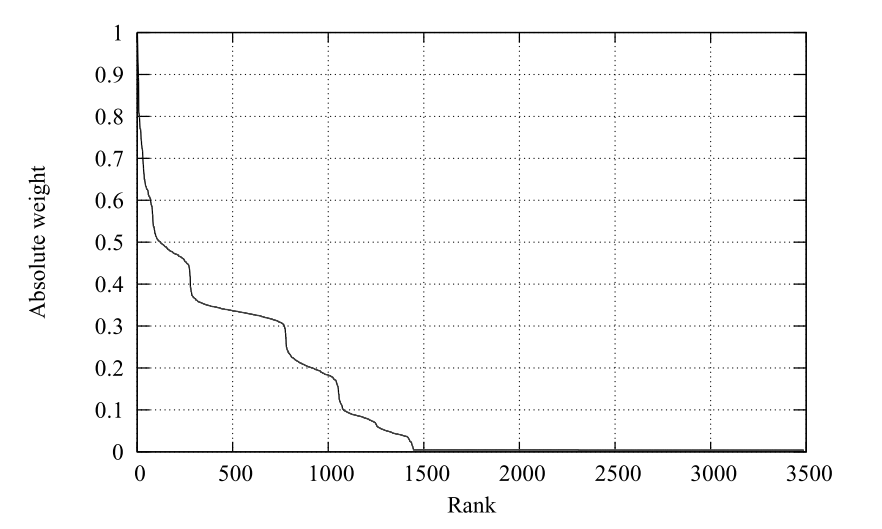
\includegraphics[width=\textwidth]{theoretische_grundlangen/gewichte}
		\caption[Die Verteilung der absoluten Gewichte]{Die Verteilung der absoluten Gewichte. (Quelle: \citealp{Remus2010})}
		\label{fig:Gewichte}
	\end{center}
\end{figure}
%%==============================================================
\section{Deutschland und China: ein kulturübergreifender Vergleich}
%%==============================================================
Deutschland und China unterscheiden sich deutlich im kulturellem Bereich. Das heißt, dass dieser Vergleich, der in dieser Arbeit gemacht wird, nicht nur länderübergreifend sondern auch kulturübergreifend ist.

Unter den vielen verschiedenen Möglichkeiten, wie die Kultur von Forschern klassifiziert wurde, sind die Theorie von \citet{hofstede2001culture} unter den Forscherinnen und Forschern am meisten verbreitet und zitiert \citep{Fong2008}. \citet{hofstede2001culture} definiert die Kultur als \textbf{``the collective programming of the mind, which distinguishes the members of one group from another''} \citep[p.~9]{hofstede2001culture}. 

``Kultur'' ist ein nationales Phänomen ist, die die unterschiedlichen Verhalten und Kenntnisse der Leute in den unterschiedlichen Ländern klassifizieren kann. Studien haben, dass Kultur einen großen Einfluss, auf die Kenntnisse und Verhalten der Konsumenten hat \citep{mccort1993culture, triandis1972analysis}. In dieser Meinung machten schon viele Wirtschaftler erfolgreich. Zum Beispiel: \citet{sia2009web} hat herausgefunden, dass sich die Kultur von Online-Konsumenten die Wirksamkeit von verschiedener Vertrauen-Errichtung-Strategien auf ihren Überzeugung signifikant mäßigt. Und \citet{Mazaheri2011958} hat auch festgestellt, dass die Auswirkung von dem Inhalt der Webseite und der Attitude des Services über die Absicht vom Kaufen durch die Orientierung der Kultur der Online-Konsumenten gemäßigt sein wird.
%%============================================
\subsection{Kulturelle Dimensionen}
%%============================================
Eine Dimension ist ein Aspekt der Kultur, der sich von anderen Kulturen unterschiedet. Nach \citet{hofstede2013interkulturelle} gibt es die folgendermaße benannten Diemensionen: \emph{Machtdistanz (von gering bis groß), Kollektivismus gegenüber Individualismus, Femininität gegenüber Maskulinität, Unsicherheitsvermeidung (von schwach bis stark) und langfristige Orientierung gegenüber kurzfristiger Orientierung, Nachsicht gegenüber Beherrschtheit}. Zusammen bilden sie ein sechsdimensionales Modell von unterschiedlichen Kulturen. In diesem Modell hat jede Kultur eine Punktzahl in jeder Dimension, und die Kultur wird auch dadurch gekennzeichnet. \citep[p. ~29]{hofstede2013interkulturelle}.

In den folgenden Abschnitte \ref{dimension:machtdistanz} bis \ref{dimension:langfristig} werden diese Dimensionen detaillierter. Darüber hinaus werden die wichtigen Unterschieden in den jeweiligen Dimensionen im Bereich der \ac{OCRs} sowie Meinungen oder wirtschaftlichen Aspekten erfasst. 

Die Logik von Gesellschaften entspricht aber nicht der Logik der die Gesellschaften betrachtenden Individuen. Vielleicht scheint keine logische Notwendigkeit für die Verknüpfung von Menschen zu bestehen, aber jede Dimension erfasst eine Reihe von Phänomenen in der Gesellschaft, die empirischen Untersuchungen zufolge in Kombination auftreten. Viele verschiedene Aspekte einer Phänomene werden zusammengefasst, diese treten in Kombination, und in trennbaren Verbindungen auf. In manchen Gesellschaften oder Kulturen gibt es einen Trend oder Aspekt, das gegen den allgemeinen Trend ist, der in den meisten anderen Gesellschaften gefunden wird.\citep[p. ~29]{hofstede2013interkulturelle}
%%======================================================
\subsection{Machtdistanz} \label{dimension:machtdistanz}
%%======================================================
Nach \citet{hofstede2013interkulturelle} kann man Machtdistanz auch definieren als \emph{das Ausmaß, bis zu welchem die weniger mächtigen Mitglieder von Institutionen \ac{bzw.} Organisationen eines Landes erwarten und akzeptieren, dass Macht ungleich verteilt ist.} Institutionen wie Familie, Schule und die Gemeinschaft bilden die Hauptelemente einer Gesellschaft; unter Organisation ist der Ort zu verstehen, wo die Leute arbeiten. \citep[p. ~42]{hofstede2013interkulturelle}

%%Man kann sagen, dass die Position der Machtdistanz Menschen Auskunft über die Abhängigkeit von Beziehungen in einem Land gibt. In Ländern mit geringer Machtdistanz ist die Abhängigkeit des Mitarbeiters von seinem Vorgesetzten begrenzt, und ein konsultativer Stil wird bevorzugt. Das heißt: es gibt eine Interdependenz zwischen Mitarbeiter und Vorgesetztem. Die emotionale Distanz zwischen ihnen ist gering: für den Mitarbeiter ist der Vorgesetzte immer ansprechbar und er traut sich auch, ihm zu widersprechen. In Ländern mit großer Machtdistanz stellt man eine große Abhängigkeit des Mitarbeiters von seinem Vorgesetzten fest. Die Mitarbeiter reagieren, indem sie diese Abhängigkeit vorziehen (autokratischer oder patriarchalischer Vorgesetzter) oder völlig ablehnen. In der Psychologie wird dieses Verhalten Kontradependenz genannt: Das heißt Abhängigkeit, aber mit negativen Vorzeichen. Bei Ländern mit starker Machtdistanz stößt man auf eine Polarisierung zwischen Abhängigkeit und Kontradependenz. In diesem Fall ist die emotionale Distanz zwischen Mitarbeiter und Vorgesetzten sehr groß: die Mitarbeiter sprechen nur sehr selten ihren Vorgesetzten direkt an \ac{bzw.} widersprechen ihm.  \citep[p. ~41]{hofstede2013interkulturelle}
\begin{table}[htb]
    \centering
    \begin{tabularx}{\textwidth}{X X}
        \hline
        Geringe Machtdistanz     & Große Machtdistanz     \\ \hline
        Ungleichheit unter den Menschen sollte so gering wie möglich sein.         & Ungleichheit unter den Menschen wird erwartet und ist erwünscht.            \\ \hline
        Tendenz zu Dezentralisation.         & Tendenz zu Zentralisation.             \\ \hline
	Mitarbeiter erwarten, in Entscheidungen miteinbezogen zu werden. & Mitarbeiter erwarten, Anweisung zu erhalten. \\ \hline
	Der Einsatz von Macht muss legitimiert sein und wird danach beurteilt, was gut und was böse ist. & Macht geht vor Recht. Wer die Macht hat, ist legitimiert dazu und ist gut. \\ \hline
	Alle haben die gleichen Rechte. & Die Mächtigen genießen Privilegien. \\ \hline
	Hierarchische Struktur in einer Organisation bedeutet eine ungleiche Rollenverteilung aus praktischen Gründen. & Hierarchische Struktur in Organisationen sind ein Spiegelbild einer Ungleichheit von Natur aus zwischen oberer und unterer Schicht. \\ \hline
	Die vorherrschenden Religionen und die philosophischen Systeme betonen die Gleichheit & Hierarchie und Einteilung der Gesellschaft in Klassen wird von Religion und philosophischer Gedankenwelt begünstigt. \\ \hline
	Ausgeprägte Parteienlandschaft. Parteien der Mitte sind stark, extreme Links- und Rechtsparteien schwach. & Parteienspektrum schwach ausgeprägt. Schwaches Zentrum, starke Links- und Rechtsparteien. \\ \hline
    \end{tabularx}
	\caption[Die wichtige Unterschiede zwischen Gesellschaften mit geringer und großer Machtdistanz]{Die wichtige Unterschiede zwischen Gesellschaften mit geringer und großer Machtdistanz (Quelle: in Anlehnung an \citealp[p. ~52, 57]{hofstede2013interkulturelle})}
	\label{tab:machtdistanz}
\end{table}

Tabelle \ref{tab:machtdistanz} zeigt die wichtigen Unterschiede von \citeauthor{hofstede2013interkulturelle} zwischen Gesellschaften mit geringer und großer Machtdistanz. Diffusionsforschung hat eine negative Beziehung zwischen der Bewertung von Machtdistanz und der Diffusionsrate des Produkts festgestellt \citep{van2003effect, yeniyurt2003does}. \citet{smith1995rotter} zeigen, dass Kulturen mit geringer Individualismus und hohe Machtdistanz tendenziell eine geringere interne Kontrollüberzeugung haben. Diese Befunde legen nahe, dass Machtdistanz einen negativen Einfluss auf Produktdiffusion und -bewertung haben.

In Kulturen mit starker Machtdistanz, sind Ungleichheiten in der Gesellschaft erwartet. Diese Erwartung fördert die Vorstellung, dass Informationsaustausch auch ungleich ist. Die Mächtigen erwarten, dass mehr Informationen als Menschen mit weniger Macht zu halten. Diejenigen, die in der Machtdistanz eine geringe Punktzahl sind, geben ihre Ideen und Ansichten zum anderen eher, weil sie dazu neigen, jeden als gleich anzusehen. Diejenigen, die in hohen Machtdistanzpunkten sind, zeigen sich zurückhaltender in ihren Gruppeninteraktionen, vor allem im Umgang mit Menschen, die mächtiger sind. Ungleichheit der Macht fordert Mitglieder mit unterschiedlichen Machtsstufen zu verschiedenen Gruppen. In diesem Umfeld entsteht mehr Interaktionen (zum Beispiel: \ac{OCRs}) mit denen, die zu den gleichen Machtsstufen gehören. \citep{Lam2009} 

Es gibt noch einige Unterschiede dazwischen, aber sie sind nicht so wichtig in diesem Bereich, welche diese Arbeit studiert. In Zusammenhang mit \ac{OCRs} gibt es von Kunden und Verkäufern, und zwischen Kunden unterschiedliche Machtdistanz in verschiedenen Kulturen. Dazu beeinflusst diese Dimension die Inhalte und die Polarität der Gefühle in den \ac{OCRs} groß.
%%======================================================
\subsection{Individualismus gegenüber Kollektivismus}
%%======================================================
Die als Individualismus gegenüber Kollektivismus bezeichnetet Dimension ist folgendermaßen definiert: \emph{Individualismus beschreibt Gesellschaften, in denen die Bedingung zwischen den Individuen locker sind: man erwartet von jedem, dass er für sich selbst und seine unmittelbare Familie sorgt. Sein Gegenstück, der Kollektivismus, beschreibt Gesellschaften, in denen der Mensch von Geburt an in starke, geschlossene Wir-Gruppen integriert ist, die ihn ein Leben lang schützen und dafür bedingungslose Loyalität verlangen.} \citep[p. ~67]{hofstede2013interkulturelle}

Nachfolgende Forschung von \citet{grennfield2000approaches} betrachtet, dass diese Dimension die ``Tiefenstruktur'' unter diesen sechs Dimensionen ist, und einige weitere Studien \citep{sia2009web, triandis2001individualism} stellen vor, dass es die wichtigste Dimension ist, um die Unterschiede verschiedener Gesellschaften oder Nationen zu erklären.

Diese Dimension ist vielleicht die am häufigsten verwendete Dimension der kulturellen Variabilität der kulturübergreifenden Verbraucherforschung \citep{aaker1997effect, han1994persuasion}. Mitglieder einer individualistischen Kultur, sowie der USA, neigen dazu, sich selbst als unabhängig von anderen, und sich auf Eigenständigkeit, interne Attribute, Getrenntheit und Entfernung von in-Gruppen zu betrachten \citep{singelis1994measurement}. Im Gegensatz dazu, betonen die Mitglieder in einer kollektivistischen Kultur wie China und Korea die Interdependenz und Wert auf ein harmonisches Arrangement, soziale Normen, Verbundenheit und in-Gruppenmitgliedschaften \citep{singelis1994measurement}.

\citeauthor{hofstede1998masculinity} hat auch herausgefunden, dass diese Dimension, Kollektivismus gegenüber Individualismus, die Wahl und Entscheidungsfindung des Verbrauchers beeinflusst. Entscheidungen über das Konsumverhalten sind selten rein individuell. In kollektivistischen Kulturen, werden individuelle Entscheidungen im Konsens mit der Gruppe gemacht und es gibt keine rein individuelle Entscheidungen zu treffen.\citep[p. ~65]{hofstede1998masculinity}

In kollektivistischen Kulturen, sind die Menschen eher sich selbst in Bezug auf die Gruppenmitgliedschaft zu berücksichtigen und legen an erster Stelle das Wohl \citep{triandis1994theoretical}. Im Gegensatz dazu sind die Menschen in individualistischen Kulturen eher selbst als autonome zu denken und machen die individuellen Interessen an erster Stelle \citep{shweder1990defense}. In kollektivistischen Kulturen sind die nicht-lebensbedrohenden Verletzungen der sozialen Verantwortung eher moralisch betrachtet, während sie als Dinge der persönlichen Wahl in individualistischen Ländern zu betrachten ist \citep{miller1990perceptions}. In individualistischen Kulturen haben die persönlichen Ziele in der Regel Vorrang vor Gruppenziele, aber in kollektivistischen Kulturen sind eher die Gruppenziele im Vordergrund \citep{triandis1994theoretical}.

Im Bereich \ac{OCRs} oder \ac{eWOM} haben Studien bisher noch wenige Ergebnisse. \citet{Luo2014} haben herausgefunden, dass durch die stärkere Wirkung der zweiseitigen Informationen (im Vergleich zu einseitigen Informationen) die Wahrnehmung von Glaubwürdigkeit der Informationen der \ac{eWOM} Leser gestärkt wird, wenn die Leser mit individualistischen Kulturen sind, verglichen mit denen, die mit kollektivistisch kulturellen Orientierung sind. Je höher kollektivistische Kultur die \ac{eWOM} Leser bekennen, desto stärker wirken sich die Informationskonsistenz und die Informationsbewertung auf ihre Wahrnehmung von Informationsglaubwürdigkeit. 
%%======================================================
\subsection{Maskulinität gegenüber Femininität}
%%======================================================
Nach \citet{hofstede2013interkulturelle}, ist diese Dimension Femininität gegenüber Maskulinität zu nennen, da \emph{diese Dimension die einzige ist, bei der die männlichen und die weiblichen Angestellten von IBM durchweg verschiedene Punktwerte erzielten}. Nur bei der Dimension wurde ein solcher Unterschied unter den Geschlechtern festgestellt. \citep[p. ~101]{hofstede2013interkulturelle}

``Legt man die Informationen über Unterschiede zwischen Gesellschaften bei dieser Dimension zugrunde, so kommt man zufolgender Definition: \emph{Maskulinität} kennzeichnet eine Gesellschaft, in der die Rollen der Geschlechter klar gegeneinander abgegrenzt sind: Männer haben bestimmt, hart und materiell orientiert zu sein, Frauen müssen bescheidener sensibler sein und Wert auf Lebensqualität legen. \emph{Femininität} kennzeichnet eine Gesellschaft, in der sich die Rollen der Geschlechter überschneiden: sowohl Frauen als auch Männer sollten bescheiden und feinfühlig sein und Wert auf Lebensqualität legen.'' \citep[p. ~101]{hofstede2013interkulturelle}

Feminine Kulturen werden durch eine stärkere Beziehungsorientierung gekennzeichnet. Für sie sind die Lebensqualität und die Menschen wichtiger. Sie betonen, wer eine Person ist, und sie arbeiten, um nicht als die andersherum zu leben. \citep{Schumann2010a}

Maskuline Kulturen werden durch einen stärkeren Ego-Orientierung gekennzeichnet, so dass die Menschen sich selbst und ihre Daseinsberechtigung nach ihrer Arbeit und Geld oder Gegenstände definieren \citep{Schumann2010a}. Wegen der materialistischen und Besitz orientierten Charakter der maskulinen Kulturen haben Forscher vorgeschlagen und fand Beweise für die höheren Ebenen der Informationsaustausch sowie Informatonserfassungsaktivitäten \citep{dwyer2005exploratory, Lam2009, liu2001relationships}. Gegenstände sind in maskulinen Kulturen hoch geschätzt, weil sie Erfolg und Status widerspiegeln. Menschen definieren sich viel mehr durch ihren Besitz und deshalb legen sie mehr Nachdruck auf die Information mit diesen Beziehungen \citep{dwyer2005exploratory}. 

Foscher haben daswegen vorgeschlagen, dass die Maskulinität Einflüsse auf die Erzeugung und Auswirkung der \ac{WOM} haben, aber diese Hypothese wird nicht durch die Ergebnisse gestützt \citep{Schumann2010a, Lam2009}. Das heißt, dass es noch keine direkte Beweise gibt, dass \ac{WOM} \ac{bzw.} \ac{OCRs} sich bislang zwischen maskulinen und femininen Kulturen unterschieden lassen.
%%======================================================
\subsection{Unsicherheitsvermeidung}
%%======================================================
``Unsicherheitsvermeidung lässt sich daher definieren als der \emph{Grad, in dem die Mitglieder einer Kultur sich durch ungewisse oder unbekannte Situationen bedroht fühlen.}'' Unsicherheitsvermeidung ist ein Gefühl, das unter anderem in nervösem Stress bringt, und dieses Gefühl fordert geschriebenen oder ungeschriebenen Regeln. \citep[p. ~133]{hofstede2013interkulturelle}

Kulturen mit starker Unsicherheitsvermeidung werden durch die Notwendigkeit gekennzeichnet, um Unklarheiten und Risiken zu reduzieren \citep{kale1992understanding}. Verglichen mit Menschen in Kulturen mit niedriger Unsicherheitsvermeidung, nehmen die Mitglieder der hohen Unsicherheitsvermeidung, das Leben mehr als eine Bedrohung wahr, und erleben höhere Ebenen der Angst. Um diese Angst zu senken, werden sie stärker motiviert, um die wahrgenommene Zweideutigkeit und Unsicherheit des Lebens zu reduzieren \citep{doney1998understanding}. Ein Weg um die Unklarheiten und Unsicherheiten zu reduzieren, ist die Beratung oder Zusicherung von vertrauenswürdigen anderen zu suchen. Im Einklang mit dieser Vorstellung wird eine hohe Unsicherheitsvermeidung mit einem höheren Niveau der Meinungsaustausch sowie Meinungsssucht verbunden sein \citep{Lam2009, liu2001relationships, dawar1996cross, money1998explorations}. Die Menschen in Kulturen mit hoher Unsicherungsvermeidung werden es auch versuchen, sich so in bereits vorhandenen geschäftlichen Beziehungen zu verhalten, weil sie ihre Meinung über die Verkäufer versichern wollen \citep{Schumann2010a}.

Personen in Kulturen mit niedriger Unsicherungsvermeidung haben größeren Glauben, dass sie ihr eigenes Leben und die Welt im Allgemeinen beeinflussen können \citep{hofstede2001culture}. Daher sind sie für das Informationserfassungsverhalten weniger engagiert und sollten weniger anfällig gegen äußere Einflüsse auf ihr Konsumverhalten und Erkenntnisse sein \citep{dawar1996cross, money1998explorations}. 

\citet{Schumann2010a} haben auch herausgefunden, dass die Auswirkung der \ac{WOM} größer für die Kunden in Kulturen mit hoher Unsicherheitsvermeidung als die mit niedriger Unsicherheitsvermeidung ist. \citet{liu2001relationships} haben herausgefunden, dass mit schlechtem Service, Personen aus geringerer Unsicherheitsvermeidungskulturen häufiger sagten, dass sie wechseln wollen, negegative Kommentaren geben, oder sich darüber beschweren, als die Personen in Kulturen mit höherer Unsicherheitsvermeidung. \citet{donthu1998cultural} zeigen, dass die Menschen in Kulturen mit hoher Unsicherheitsvermeidung im Allgemeinen positivere Kommntaren schreiben oder geben, als die mit niedriger Unsicherheitsvermeidung.
%%======================================================
\subsection{Langfristige Orientierung gegenüber kurzfristige Orientierung} \label{dimension:langfristig}
%%======================================================
Langfristige Orientierung gegenüber kurzfristiger Orientierung, als eine Dimension, machte man relativ neu von Unterschieden zwischen nationalen Kulturen aus \citep[p. ~29]{hofstede2013interkulturelle}. Diese Dimension ist auch als die Konfuzianische Dynamik genannt \citep{hofstede2013interkulturelle, Schumann2010a, Lam2009}. Man kann folgende Werte am Pol, der `langfristige Orientierung' bezeichnen: \citep[p. ~190]{hofstede2013interkulturelle}
\begin{itemize}
  \item Ausdauer (Beharrlichkeit)
  \item Ordnung der Beziehungen nach dem Status
  \item Einhaltung dieser Ordnung
  \item Sparsamkeit
  \item Schamgefühl
\end{itemize}

Am entgegengesetzten Pol, der `kurzfristigen Orientierung':
\begin{itemize}
  \item Persönliche Standhaftigkeit und Festigkeit
  \item Wahrung des `Gesichts'
  \item Respekt vor der Tradition
  \item Erwiderung von Gruß, Gefälligkeiten und Geschenken
\end{itemize}

Die Wert des einen Pols sind eher auf die Zukunft hin ausgerichtet (insbesondere Beharrlichkeit und Sparsamkeit), und eher dynamisch. Dagegen sind mehr auf die Vergangenheit und Gegenwart hin ausgerichtet, und eher statisch. \citep[p. ~190]{hofstede2013interkulturelle}

\citet{Yoon2009} hat herausgefunden, dass der Interaktionseffekt des Vertrauen $\times$ langfristige Orientierung erhebliche Auswirkungen auf die Verwendungsabsicht hat. Aber die langfristige Orientierung hat keine direkte Wirkung auf die Verwendungsabsicht. Deshalb glaubte \citeauthor{Yoon2009}, dass langfristige Orientierung ein reiner Moderator des Vertrauens und der Verwendungsabsicht war. Das heißt: Je höher der Grad der langfristigen Orientierung ist, desto stärker ist die Wirkung des Vertrauens auf die Verwendungsabsicht. \citep{Yoon2009}

In langfristig orientierten Gesellschaften suchen die Menschen die Tugend, während kurzfristig orientierte Gesellschaften daran glauben , die absoluten Wahrheit festzustellen \citep{Sohaib2014}. Im Vergleich zu langfristig orientierten Konsumenten, erfahren die kurzfristig orientierten Konsumenten weniger wahrgenommene Kontrolle in unbefriedigenden Service-Begegnungen, und Entschädigung hätten einen stärkeren Effekt auf ihnen \citep{Hui2001161, patrick2004attributions}.
%%=========================================================== 
\subsection{Nachsicht gegenüber Beherrschtheit}
%%=========================================================== 
Die sechste Dimension, Nachsicht gegenüber Beherrschtheit, wird auf Englisch ``Indulgence versus Restraint'' genannt. Diese Dimension ist ganz neu und wurde in dem Jahr 2010 in das Modell von Hofstede angelegt \citep[p.~ 285]{hofstede2010cultures}. 

Die Definition nach \citet{hofstede2010cultures} ist folgende: \emph{``Indulgengce (Nachsicht) stands for a tendency to allow relatively free gratification of basic and natural human desires related to enjoying life and having fun. Restraint (Beherrtheit) reflects a conviction that such gratification needs to be curbed and regulated by strict social norms.''}

Eine Umfrage in 2002-03 wurde durch Pew Research Center darüber gemacht, ob die ausländischen Filmen und Musik gut sind. Die Befragten, welche ``sehr gut'' geschrieben haben, sind positiv abhängig von der Nachsicht. Es wurde auch herausgefunden, dass nachsichtigere Gesellschaften mehrere Leute haben, die die Importierung von Entertainment bevorzugen. \citep[p.~292]{hofstede2010cultures}

\citet{kuppens2006universal} haben herausgefunden, dass Menschen, die in einer nachsichtigen Kultur sind, sich gerne an positiven Gefühlen erinnern. \citet{schimmack2002cultural} haben einen ähnlichen Ergebnis gefunden. In der Forschung berichten die Studenten mehr, die in nachsichtigerer Kultur sind, wenn sie positive Erfahrung haben. Durch den Vergleich der hoch und niedrig nachsichtigen Teiproben, finden \citet{Zhou2015}, dass Nachsicht die Wirkung des utilitaristischen Wert schwächt, und die Wirkung von hedonischen Wert auf affektivem Engagement stärkt. 

Es gibt schon viele Forschungen im Bereich Online-Kaufen oder Kaufverhalten, die oft auf den Spontankauf fokussieren \citep{sharma2005self}. Im Bereich \ac{eWOM} oder \ac{OCRs}, gibt es noch wenige Ergebnisse.

\citet{Mangold1999wom} geben einen Einblick, um die Gründe, warum Menschen nachsichtig in \ac{eWOM}-Kommunikationen sind, zu verstehen. Aber dieses Ergebnis betrifft keine Dimension von \citeauthor{hofstede2013interkulturelle}.

%%===========================================================
\subsection{Das sechsdimensionale Modell für Deutschland und China} \label{6dimensionaleModell}
%%===========================================================
Basierend auf diesem sechsdimensionalen Modell, kann man erkennen, dass Deutschland und China viele Unterschiede in der Kultur haben. Nach der Forschung von \citet{hofstede2001culture, Singh2006, Cyr2014}, unterschieden sich die Kulturen in Deutschland und China deutlich. Abbildung \ref{fig:sechsdimensionen} zeigt die Ungleichheiten zwischen Deutschland und China im sechsdimensionalen Modell.

\begin{figure}[htb]
	\begin{center}
		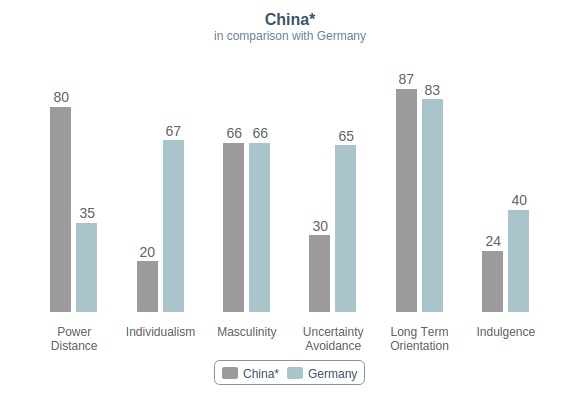
\includegraphics[width=\textwidth]{theoretische_grundlangen/sechsdimensionen}
		\caption[Das sechsdimensionale Modell für Deutschland und China]{Das sechsdimensionale Modell für Deutschland und China (Quelle: \citealp{HofstedeWebseite})}
		\label{fig:sechsdimensionen}
	\end{center}
\end{figure}

Verglichen mit deutschen Menschen, haben die Chinesen größere Machtdistanz. Das heißt: die Ungleichheit ist überall, erwartet und erwünscht, nicht nur zwischen den Konsumenten und den Verkäufer im Internet, sogar auch in den Konsumenten untereinander. Die deutsche Kultur ist individualistisch aber die chinesische ist typisch kollektivistisch. Es wird vorgeschlagen, dass die deutschen Konsumenten sich unabhängiger von anderen verhalten, als die Chinesen. Die chinesischen Konsumenten verhalten sich mehr zentralisiert. In Dimensionen ``Maskulinität gegenüber Femininität'',``Langfristige Orientierung gegenüber kurzfristige Orientierung'' und ``Nachsicht gegenüber Beherrschtheit'' sind Deutschland und China auf gleicher Ebene. Aber bei der Unsicherheitsvermeidung ist ein großer Spalt. Nach \citet{donthu1998cultural}, wird es vorgeschlagen, dass die Deutschen positivere Kommentaren schreiben wollen, als die Chinesen. 

%%===========================================================
\section{Relevante Forschungsergibnisse zum Textileinzelhandel} \label{sec:relevante_forschungen}
%%===========================================================

Im Bereich Textileinzelhandel oder \acl{OCRs} gibt es schon viele Forschungen, aber die kulturübergreifenden Forschungen in diesem Bereich sind wenig (nur 8). Die meisten vergleichen die Kulturen zwischen Osten (meistens China) und Western. Fünf Forschungen haben das Modell von \citet{hofstede2001culture} genutzt. Tabelle \ref{tab:relevanteForschungen} zeigt die relevanten kulturübergreifenden Forschungen im Bereich \acl{OCRs}.

\begin{table}[h]
\centering
\begin{longtable}{p{.08\textwidth} p{.20\textwidth} p{.22\textwidth}  p{.40\textwidth}}
  \hline
  Quelle& Verfahren von Kultur& Länder/Bereich &Ergebnisse \\ \hline
  \citet{Adams2005} & Dimension: Individualismus gegenüber Kollektivismus genutzt &Großbritannien, China/eBusiness & Unterschiede in der Benutzer-Praktiken und Umgebung weisen hin, dass die E-Commerce-Geschäftsmodellen für den Westen nicht ganz geeignet für den Osten sein können. \\ \hline
  \citet{Chu2011} & Dimension: Individualismus gegenüber Kollektivismus genutzt &USA, China/Soziale Netzwerke & Nationale Kultur spielt einen wesentlichen Faktor, der Engagement der Verbraucher in \ac{eWOM} in sozialen Netzwerken, die beide Länder betrifft. \\ \hline
  \citet{Fong2008} & Dimension: Individualismus gegenüber Kollektivismus genutzt & USA, China/Ursprungsland-Effekte& China-basierte Diskussionsforen engagieren in höheren Ebenen der Informationssuche und niedrigere Informationshingabe als in den USA. \\ \hline
  \citet{Jin2010}& keine Dimension von \citeauthor{hofstede2001culture} genutzt& India, China/Kleidungen & Chinesische und indische Verbraucher bewerten Attribute von Kleidungen unterschiedlich. \\ \hline
  \citet{lu2015understanding}& keine Dimension von \citeauthor{hofstede2001culture} genutzt& USA, China/Kleidungen & Chinesische und amerikanische Verbraucher bewerten Attribute von Kleidungen unterschiedlich. \\ \hline
 %% \citet{Luo2014}& Dimension: Individualismus gegenüber Kollektivismus genutzt & 
  \citet{Singh2006} & Alle Dimensionen von \citeauthor{hofstede2001culture} genutzt& Deutschland, India, China/Wahrnehmung der Webseite-Anpassung von Verbrauchern& Kultur spielt eine große Rolle, um die Verbraucher der Webseite anzupassen. Und Kultur beeinflusst Glauben, Meinungen und Kaufabsicht der Verbraucher im Internet. \\ \hline
  \citet{Sohaib2014} & 4 Dimensionen (außer langfristiger Orientierung und Nachsicht) von \citeauthor{hofstede2001culture} getestet. &Pakistan und Australien/\acs{B2C}-Webseite & \acs{B2C}-Webseite spiegeln das kulturelle Umfeld, das die Online-Käufer umgibt. Es scheint dass die Kultur die Kaufabsicht von Online-Käufer beeinflusst. \\ \hline
  \citet{Stenberg2014} & Unsicherheits-vermeidung und Individualismus werden verwendet & Schweden und China/Kleidung & Die Hauptunterschiede waren die wahrgenommene allgemeine Nützlichkeit von Online-Shopping und der Risikograd, den Verbraucher beim Online-Shopping wahrgenommen haben. \\ \hline

\caption[Die relevanten kulturübergreifenden Forschungen]{Die relevanten kulturübergreifenden Forschungen}
\label{tab:relevanteForschungen}
\end{longtable}
\end{table}


Von dieser Tabelle kann man sehen, dass es Unterschiede gibt, nicht nur zwischen Osten und Westen, sondern auch zwischen unterschiedlichen östlichen Ländern (India und China). Deshalb wird es vorgeschlagen: Aufgrund der Einflüssen von Kulturen, verhält man sich unterschiedlich, und man hat verschiedene Meinungen, wenn die Dimensionen der eigenen Kultur zueinander verschieden sind. Diese Unterschiede kann man auch in den \ac{OCRs} finden.

Im Bereich Textileinzelhandel gibt es schon einige Ergebnisse über die \ac{OCRs}, aber die meisten Ergebnisse sind über die chinesischen Verbrauchern. \citet{rahman2010evaluative} haben gefunden, dass die chinesischen Befragten mehr befasst mit funktioneller Eigenschaft waren, während die Kanadier sich mehr auf ästhetische Attribute konzentrierten. \citet{Jin2010} erklärten, dass die Verarbeitung und Passform am wichtigsten für die US-Verbraucher sind, aber nicht für die chinesischen Verbraucher. \citet{hsu2002clothing} machten einen Vergleich zwischen den Studenten in Taiwan und den USA, und stellten fest, dass die Flexibilität und Angemessenheit die wichtigen Bewertungskriterien von Kleidungen für die Studenten in Taiwan waren, nicht in den USA, aber Komfort und Passform waren für die Verbraucher aus beiden Ländern am wichtigsten. \citet{zhang2002casual} haben entdeckt, dass Passform und Komfort die wichtigsten Faktoren für die chinesischen Verbraucher mit Stil, Farbe und Verarbeitung.

Viele Studien fanden auch, dass die äußere Attribute wie Marken relativ mehr wichtig für die chinesischen Verbraucher waren. Zum Beispiel: \citet{chun1998differences} schlug vor, dass die chinesischen Verbraucher durch Markenloyalität gekennzeichnet waren und \citet{zhou2003symbolic} fanden auch, dass symbolische Attribute wichtiger als Performance zur Kaufabsicht der chinesischen Konsumenten waren. Die ``Kollektivismus'' Kultur macht die chinesischen Verbraucher mehr Sorgen um andere Meinungen und sozialen Selbstbewusstsein \citep{rahman2010evaluative}.

%%====================================================
\section{Hypothesen} \label{sec:hypothese}
%%====================================================
Wie es in dem Abschnitt \ref{SAkernprozess} beschrieben wird, wird jede Review von den Kunden als ein Dokument durch die Sentiment Analyse analysiert. Das heißt: jede Review hat eine eigene Polarität. Ähnlich wie die quantitativen \ac{OCRs}, hat das qualitative Online Review auch deswegen folgende Attribute:
\begin{description}
	\item[Volumen:] Dieses Attribut für die quantitativen \ac{OCRs} ist die Anzahl der Kommentare, die das Produkt hat \citep{Shrihari2012}. Aber hier in dieser Arbeit, beschreibt das Volumen die Anzahl der Zeichen, die der Kunde in dem qualitativen Online Review geschrieben hat.
	\item[Valenz:] Dieses Attribut für die quantitativen \ac{OCRs} ist die Anzahl Sterne, die der Kunde gegeben hat \citep{Shrihari2012}. Aber in dieser Arbeit, beschreibt die Valenz die Polarität, welche die qualitative Online Review durch die Sentiment Analyse hat.
\end{description}

Deshalb hat ein Online Review (inklusiv quantitativer und qualitativer Seite) die Attribute: Valenz der Sterne, Valenz der Polarität durch Sentiment Analyse, und Volumen von Zeichen. Für ein Produkt, gibt es viele Reviews, deswegen haben die qualitativen \ac{OCRs} für ein Produkt oder mehrere Produkte noch folgende Attribute:
\begin{description}
	\item[Varianz:] Dieses Attribut beschreibt den Grad der Polaritätsverschiedenheiten von Kunden durch die Sentiment Analyse.
	\item[Korrelationskoeffizient:] Dieser zeigt den Grad des Zusammenhangs zwischen quantitativen und qualitativen \ac{OCRs}.
\end{description}

\begin{table}[htb]
\centering
\resizebox{\textwidth}{!}{%
\begin{tabular}{|l|l|l|}
\hline
                        & quantitative \ac{OCRs}                            & qualitative \ac{OCRs}                                \\ \hline
Volumen                 & Anzahl der \ac{OCRs}                              & Anzahl der Kennzeichen                                 \\ \hline
Valenz                  & Zahl der Sterne                                   & Zahl der Polarität                                   \\ \hline
Varianz      & Grad der Meinungsverschiedenheiten                  & Grad der Polaritätenverschiedenheiten                  \\ \hline
Korrelationskoeffizient & \multicolumn{2}{l|}{der Grad des Zusammenhangs zwischen quantitativen und qualitativen \ac{OCRs}} \\ \hline
\end{tabular}
}
\caption[Die Attribute der quantitativen und qualitativen OCRs]{Die Attribute der quantitativen und qualitativen \ac{OCRs} (Quelle: eigene Darstellung)}
\label{tab:AttributeOCRs}
\end{table}

Weil die deutschen und chinesischen \ac{OCRs} gleichzeitig quantitativen und qualitativen Inhalte haben, besitzen die Attribute Valenz, Volumen, und Varianz für die quantitativen und qualitativen Aspekte unterschiedliche Bedeutungen. Tabelle \ref{tab:AttributeOCRs} zeigt dies Unterschiede.

Diese Attribute beschreiben die \ac{OCRs} mathematisch und statistisch. Basierend auf diesen mathematischen und statistischen Maßen kann man einfach einige statistischen Analysen durchführen.

Aus der Abbildung \ref{fig:sechsdimensionen} kann man deutlich sehen, dass Deutschland und China sich in Bezug auf Machtdistanz, Individualismus gegenüber Kollektivismus und Unsicherheitsvermeidung unterscheiden. Für die anderen drei Dimensionen sind Deutschland und China in gleicher Ebene, deshalb wird vorgeschlagen, dass die Dimensionen ``Maskulinität gegenüber Femininität'', ``langfristige Orientierung gegenüber kurzfristiger Orientierung'' und ``Nachsicht gegenüber Beherrschtheit'' wenige Einflüsse haben, um die deutschen und chinesischen \ac{OCRs} zu unterscheiden.

Wenn es keine kulturellen Einflüsse auf das Schreiben der \ac{OCRs} geben würde, wäre jede Erzeugung eines Online Reviews individuell und hätte keine Abhängigkeit mit anderen. Das heißt: Das Gefühl von jedem Kunden für das Produkt ist unabhängig voneinander, und die Polaritäten durch Sentiment Analyse sollte die Normalverteilung angepasst werden. %Aber es gibt in tatsächlicher Hinsicht kulturelle Einflüsse darauf. 
Deshalb wird es als die Nullhypothese $H_0$ vorgeschlagen:

\begin{description}
    \item[Hypothese $H_0$] \emph{Es gibt keine kulturelle Einflüsse auf die \acl{OCRs} an sowohl der quantitativen Seite als auch der qualitativen Seite.}
\label{hyp:0}
\end{description}

Wie in dem Abschnitt \ref{dimension:machtdistanz} beschrieben, sind die Menschen in den Kulturen mit großer Machtdistanz zurückhaltend wenn es um den Informationsaustausch nach \citet{Lam2009} geht. Nach \citet{Lam2009, liu2001relationships, dawar1996cross, money1998explorations} wird eine hohe Unsicherheitsvermeidung mit einem höheren Niveau des Meinungsaustausches sowie Meinungsssucht verbunden sein. Das heißt: %Aber die Interaktionen zwischen Menschen in den gleichen Machtstufen werden mehr sein. Bei der kollektivistischen Kultur ist das Verhalten ``alle machen, dann mache ich auch'' normal. Es entstehen Motive, eine Review für das Produkt zu schreiben, wenn das Produkt schon viele Reviews hat. Aber die Motivation ist nicht stark genug für eine lange Review. 
\begin{hyp} 
Das Volumen von chinesischen quantativen und qualitativen \acl{OCRs} ist kleiner als das von Deutschen.
\label{hyp:1}
\end{hyp}

Nach \citet{liu2001relationships} und \citet{donthu1998cultural}, geben die Menschen in Kulturen mit hoher Unsicherheitsvermeidung im Allgemeinen positivere Kommentare, als die mit niedriger Unsicherheitsvermeidung. Deshalb wird vorgeschlagen:
\begin{hyp} 
Die deutschen qualitativen und quantitativen \acl{OCRs} haben größere Valenzen als die chinesischen.
%aber die deutsche Valenz von quantitativen \ac{OCRs} ist kleiner als die chinesische Valenz im Durchschnitt.
%Und die deutschen \ac{OCRs} haben einen größere Korrelationskoeffizient zwischen quantitativen und qualitativen \ac{OCRs} als die Chinesischen.
\label{hyp:2}
\end{hyp}

Ungleichheit unter den Menschen in Kulturen mit großer Machtdistanz wird erwartet und ist erwünscht nach \citet{hofstede2013interkulturelle}, und hierarchische Strukturen in Organisationen sind ein Spiegelbild einer Ungleichheit von Natur aus zwischen oberen und unteren Schichten. Diese sagen, dass die Varianz von Polaritäten durch Sentiment Analyse größer sein wird, wenn Menschen in Kulturen mit großer Machtdistanz leben.

Aber beim Kollektivismus wirken sich die Informationskonsistenz und die Informationsbewertung auf ihre Wahrnehmung von Informationsglaubwürdigkeit stärker aus \citep{Luo2014}. Gemäß der Theorie der \citet{hofstede1998masculinity}, machen die Menschen in den kollektivistischen Kulturen die Kaufentscheidungen im Konsens mit der Gruppe und kaum rein individuelle Entscheidungen im Gegensatz zu den Menschen in den individuellen Kulturen \citep{singelis1994measurement}. Auf Grund der größeren Machtdistanz, gibt es die zentralisierte Tendenz, aber auf der gegenüberliegenden Seite gibt es keine solche Tendenz \citep{hofstede2013interkulturelle}. China hat eine sehr hohe Machtdistanz mit kollektivistischer Kultur, aber für Deutschland ist die Machtdistanz niedrig und die Menschen sind individuell. Es gibt unterschiedliche Einflüsse auf die chinesischen und deutschen \ac{OCRs}. Das heißt: die \ac{OCRs} werden konsistenter beim Kollektivismus sein, deswegen sollte die Varianz von Polaritäten kleiner als beim Individualismus sein.

Weil die vorherigen Forschungen vorgeschlagen haben, dass die Dimension ``Individualismus gegenüber Kollektivismus'' eine Tiefenstruktur und wichtigste Dimension ist \citep{grennfield2000approaches,sia2009web, triandis2001individualism}, wird es vermutet, dass diese Dimension einen größeren Einfluss auf die \ac{OCRs} hat, deshalb:
\begin{hyp} 
Die chinesischen Valenzen von den qualitativen und quantitativen \acl{OCRs} haben kleinere Varianzen als die Deutschen.
\label{hyp:3}
\end{hyp}


%%Gemäß der Theorie von \citet{hofstede1998masculinity}, machen die Menschen in den kollektivistischen Kulturen die Kaufentscheidungen im Konsens mit der Gruppe und kaum rein individuelle Entscheidungen. Aber die Menschen in den individuellen Kulturen machen die Kaufentscheidungen individuell \citep{singelis1994measurement}. Auf Grund der größeren Machtdistanz, gibt es die zentralisierte Tendenz, aber an der gegenüberliegenden Seite gibt es keine solche Tendenz \citep{hofstede2013interkulturelle}. China hat eine sehr hohe Machtdistanz mit kollektivistischer Kultur, aber für Deutschland ist die Machtdistanz niedrig und die Menschen sind individuell. Es gibt unterschiedliche Einflüsse auf die chinesischen und deutschen \ac{OCRs}. Deswegen wird es vorgeschlagen:
Und Menschen in der kollektivistischer Kultur sind einfacher zu beeinflussen, eine quantitative Review zu geben, aber das Gefühl ist von jedem Kunden unterschiedlich und nicht einfach übereinzustimmen. Basierend auf die Hypothesen \ref{hyp:2} und \ref{hyp:3}, wird die deutschen \ac{OCRs} positiver und individueller als die chinesischen, aber der Zusammenhang zwischen quantitativen und qualitativen \ac{OCRs} ist noch nicht in Sicht. 

\citeauthor{resnick2002trust} haben durch die Studien von Online Rückkopplungsmechanismen festgestellt, dass die Feedbacks (also die \ac{OCRs} in eBay) eine hohe Korrelation zwischen den Käufern und Verkäufern haben. Und \citeauthor{Stenberg2014} haben schon gefunden, dass die Attitüde und Absicht von Menschen in China und Schweden unterschiedlich sind. Die Aspekten, auf der man sich konzentriert, sind in den USA und China unterschiedlich \citep{lu2015understanding}. Das heißt: Die Kunden geben gleichen quantitativen \ac{OCRs} aber  haben vielleicht unterschiedliche Aspekte in den verschiedenen Kulturen. Anders gesagt, die kulturellen Einflüsse auf quantitative und qualitative \ac{OCRs} sind unterschiedlich. Um diese Unterschiedlichkeit zu verdeutlichen, wird es vorgeschlagen:
\begin{hyp} 
%%Die Dichteverteilung von deutschen Polaritäten ist ähnlich wie die Normalverteilung. Aber die Dichteverteilung von chinesischen Polartitäten ist dichter und zentraliseirter als die Normalverteilung.
Der Zusammenhang zwischen den deutschen quantitativen und qualitativen \acl{OCRs} ist stärker als der Zusammenhang von den chinesischen \acl{OCRs}.
\label{hyp:4}
\end{hyp}
